\documentclass[diplomskirad]{fer}
% Dodaj opciju upload za generiranje konačne verzije koja se učitava na FERWeb
% Add the option upload to generate the final version which is uploaded to FERWeb

\usepackage{blindtext}
\usepackage{hyperref}
\usepackage{makecell}
\usepackage{graphicx}
\usepackage{adjustbox}
\usepackage{booktabs}
\usepackage{subcaption}

%--- PODACI O RADU / THESIS INFORMATION ----------------------------------------

% Naslov na engleskom jeziku / Title in English
\title{Mobile application for Kingdomms board game}

% Naslov na hrvatskom jeziku / Title in Croatian
\naslov{Mobilna aplikacija za društvenu igru Kraljevstva}

% Broj rada / Thesis number
\brojrada{1234}

% Autor / Author
\author{Petar Belošević}

% Mentor 
\mentor{Prof.\@ Marko Čupić}

% Datum rada na engleskom jeziku / Date in English
\date{June, 2026}

% Datum rada na hrvatskom jeziku / Date in Croatian
\datum{lipanj, 2026.}

% TODO englizmi italic; Kivy
% TODO programski sustav umjeto radni okvir
%-------------------------------------------------------------------------------


\begin{document}


% Naslovnica se automatski generira / Titlepage is automatically generated
\maketitle


%--- ZADATAK / THESIS ASSIGNMENT -----------------------------------------------

% Zadatak se ubacuje iz vanjske datoteke / Thesis assignment is included from external file
% Upiši ime PDF datoteke preuzete s FERWeb-a / Enter the filename of the PDF downloaded from FERWeb
\zadatak{filename.pdf}


%--- ZAHVALE / ACKNOWLEDGMENT --------------------------------------------------

\begin{zahvale}
  % Ovdje upišite zahvale / Write in the acknowledgment
\end{zahvale}


% Odovud započinje numeriranje stranica / Page numbering starts from here
\mainmatter

% Sadržaj se automatski generira / Table of contents is automatically generated
\tableofcontents

%--- UVOD / INTRODUCTION -------------------------------------------------------
\chapter{Uvod}
\label{pog:uvod}

	% popularnost društvenih igara
	U zadnjih desetak godina svjedočimo snažnom trendu digitalizacije zabavne industrije kroz razne video i online igre, streaming servise i sličnog. No, unatoč tome društvene i kartaške igre su i dalje ostale popularne kao primjer klasičnih oblika zabave. Dapače, postoji kulturološki trend prema zabavi bez ekrana koji je dao dodatan zamah u industriji društvenih i kartaških igara~\cite{BoardGamesPopularityReport2025}. Neki od razloga zašto su društvene i kartaške igre ostale popularne kod društvenih okupljanja su kombinacija poticanja strateškog razmišljanja, žive socijalne interakcije i zabave lice-u-lice\cite{BoardGamesPopularityReport2025}. Zbog svega navedenoga industrija društvenih i kartaških igara je u 2025. bila procijenjena na 19.90 milijardi američkih dolara~\cite{BoardGamesPopularityReport2025} s procjenom godišnje stope rasta od 8.3\% do 2030. godine.
	
	% problemi - zamorno praćenje rezultata
	Iako je igranje društvenih igra mnogima zabavno iskustvo, samo iskustvo igranja ima komponente koje u nekim slučajevima mogu biti zamorne. To najčešće uključuje komplicirana pravila, proces učenja igre, složen postupak računanja bodova i praćenje stanja igre, što je pogotovo izraženo u igrama koje se znaju igrati tijekom više dana. Navedene činjenice mogu umanjiti interes potencijalnih igrača za neke igre te negativno utjecati na popularnost tih igara, iako u osnovi imaju zabavan i zanimljiv koncept.
	
	% konkretan primjer - Kraljevstva
	Primjer jedne takve igre je Kraljevstva Reinera Knizie. Igra ima zanimljiv koncept u kojem igrači na ploču postavljaju korisne, štetne i posebne resurse u obliku kartica koji se dijele te dvorce kojima mogu prikupljati postavljene resurse. Igra se sastoji od 3 runde koje su vremenski relativno kratke. No, na kraju svake runde dolazi proces računanja bodova koji je relativno zahtjevan s obzirom na trajanje jedne runde. Upravo taj segment u ovoj igri može značajno pokvariti iskustvo igranja.
	
	% moja ideja - aplikacija
	Iz ovog problema proizlazi konačan cilj ovog rada - razviti sustav koji će na jednostavan način automatizirati proces bodovanja u ovoj igri te takav sustav zapakirati u jednostavno korisničko sučelje u obliku Android mobilne aplikacije. Aplikacija treba omogućiti jednostavan prijenos informacija s igraće ploče u programski model igre te primijeniti logiku igre za izračun samih bodova. Kao najpraktičnije rješenje za unos podataka iz perspektive korisnika nalaže se fotografiranje igraće ploče. Fotografija ploče sadrži potpunu informaciju o stanju igre, a korisniku je puno jednostavnije uslikati fotografiju nego ručno upisivati pojedine elemente na ploču.
	
	% računalni vid?
	Takav pristup unosa podataka zahtijeva od sustava mogućnost detekcije ploče na fotografiji i prepoznavanje pojedinih elemenata na njoj. U tu svrhu potrebno je koristiti širok spektar metoda računalnog vida od klasičnih algoritama do dubokih konvolucijskih modela strojnog učenja. S obzirom na to da takvi algoritmi mogu griješiti, aplikacija također mora omogućiti korisniku jednostavno ispravljanje predikcija aplikacije.
	
	% cilj rada i specifičnosti
	Radi jednostavnog postavljanja ovakve aplikacije te smanjenja vanjskih ovisnosti u aplikaciji, dodatan je cilj ostvariti da aplikacija nije napravljena kao klasičan web servis, već da bude ostvarena potpuno lokalno. Zbog toga je potrebno kompletnu logiku ostvariti na način da njezina memorijska i računalna složenost bude prikladna za mobilne uređaje, koji imaju ograničene performanse i resurse u odnosu na standardna računala. 
	
	% struktura
	Za takav pothvat u ovom radu je napravljen kompletan programski sustav za izradu aplikacije i njezine pozadinske logike. U radu su detaljno razrađeni i opisani svi elementi tog procesa. Fokus ovog rada nije isključivo na konačnoj aplikaciji već na sveukupnom procesu, a on se sastoji od:
	\begin{itemize}
		\item razvoja algoritma za detekciju igraće ploče i izrezivanja pojedinih polja s ploče,
		\item izrade skupa podataka za učenje,
		\item izrade raznovrsnih metoda augmentacije slika,
		\item razvoja sustava za treniranje dubokih modela,
		\item dizajniranja i treniranja dubokih konvolucijskih modela,
		\item pisanja programskog modela pravila igre te
		\item izrade mobilne aplikacije koja enkapsulira razvijenu logiku.
	\end{itemize}

%-------------------------------------------------------------------------------
\chapter{Pregled područja}
\label{pog:pregled_podrucja}

	Danas već postoje razne pomoćne aplikacije i web-stranice za društvene igre kojima je cilj unaprijediti iskustvo igranja društvenih igra kroz različite aspekte. Većina njih nije napravljeno kao pomoć u specifičnoj igri, već služe kao generalni alat za pomoć igračima. Neki od popularnih primjera~\cite{BestBoardGameApps} navedeni su u nastavku.
	\begin{itemize}
		\item \href{https://trythesegames.com/}{\textit{Try These Games}} - web-stranica koja preporučuje nove igre na temelju preferencija igrača.
		\item \href{https://www.bgstatsapp.com/}{\textit{Board Game Stats}} - aplikacija koja prati igračeve statistike kroz razne igre, uključujući broj pobjeda, učestalost igranja i slično.
		\item \href{https://www.boardgameoracle.com/}{\textit{Board Game Oracle}} - stranica za praćenje dostupnosti i cijena pojedinih igara u različitim trgovinama.
		\item \href{https://dized.com/}{\textit{Dized Board Game Companion}} - aplikacija koja sadrži detaljne i interaktivne tutorijale za mnoge popularne igre s ciljem olakšavanja procesa učenja igranja.
	\end{itemize}
	
	Također postoje i aplikacije specijalizirane za konkretne igre. Jedan takav primjer je aplikacija \href{https://apps.apple.com/us/app/pointsman/id1447780441}{\textit{Pointsman}} namijenjena za igru \textit{Ticket To Ride}. Aplikacija je razvijena za iOS te omogućuje korisniku snimanje igraće ploče iz čega se izračunavaju ostvareni bodovi za svakog igrača. Aplikacija dakle koristi metode računalnog vida za detekciju ploče i elemenata igre te između ostalog prilagođene algoritme strojnog učenja za prepoznavanje vlakova na ploči~\cite{Pointsman}. S obzirom na to da aplikacijska logika može napraviti krive predikcije, aplikacija korisniku nudi jednostavno sučelje za potrebna ispravljanja~\cite{Pointsman}. Ova aplikacija je upravo reprezentativan primjer onoga što se želi postići u ovom diplomskom radu za društvenu igru Kraljevstva, uz značajno jednostavniji vizualni dizajn sučelja te za Android okruženje. 
			
\chapter{Društvena igra Kraljevstva}
	\label{pog:drustvena_igra}
	
	Kraljevstva su društvena igra za 2 do 4 igrača koju je dizajnirao Reiner Knizia. Igra se sastoji od 3 identične runde. U svakoj rundi igrači na ploču naizmjence postavljaju nasumične kartice ili dvorce. Igraća ploča se sastoji od pravilne rešetke od 5 redaka i 6 stupaca. Runda završava kada se zauzmu sva polja na ploči. Primjer igraće ploče s postavljenim karticama i dvorcima na kraju runde je vidljiv na slici~\ref{slk:igraca_ploca}. Na kraju runde računaju se bodovi svakog igrača te se oni u konačnici zbrajaju. Igrač s najviše bodova pobjeđuje. 
	
	Vrijedi napomenuti da se u pravoj igri bodovi prate pomoću novčića. Na početku svaki igrač dobiva novčiće u vrijednosti od 50 bodova. Kroz igru igrač dobiva ili gubi novčiće ovisno o ostvarenim bodovima. U ovom radu će spomenuti mehanizam novčića biti zanemaren, ali to neće utjecati na samu mehaniku igre. Dakle, u radu se drži pretpostavka da svaki igrač počinje s 0 bodova te da nema novčića za praćenje bodova. Bodove će se ionako moći pratiti kroz aplikaciju.
	
	\begin{figure}[htb]
		\centering
		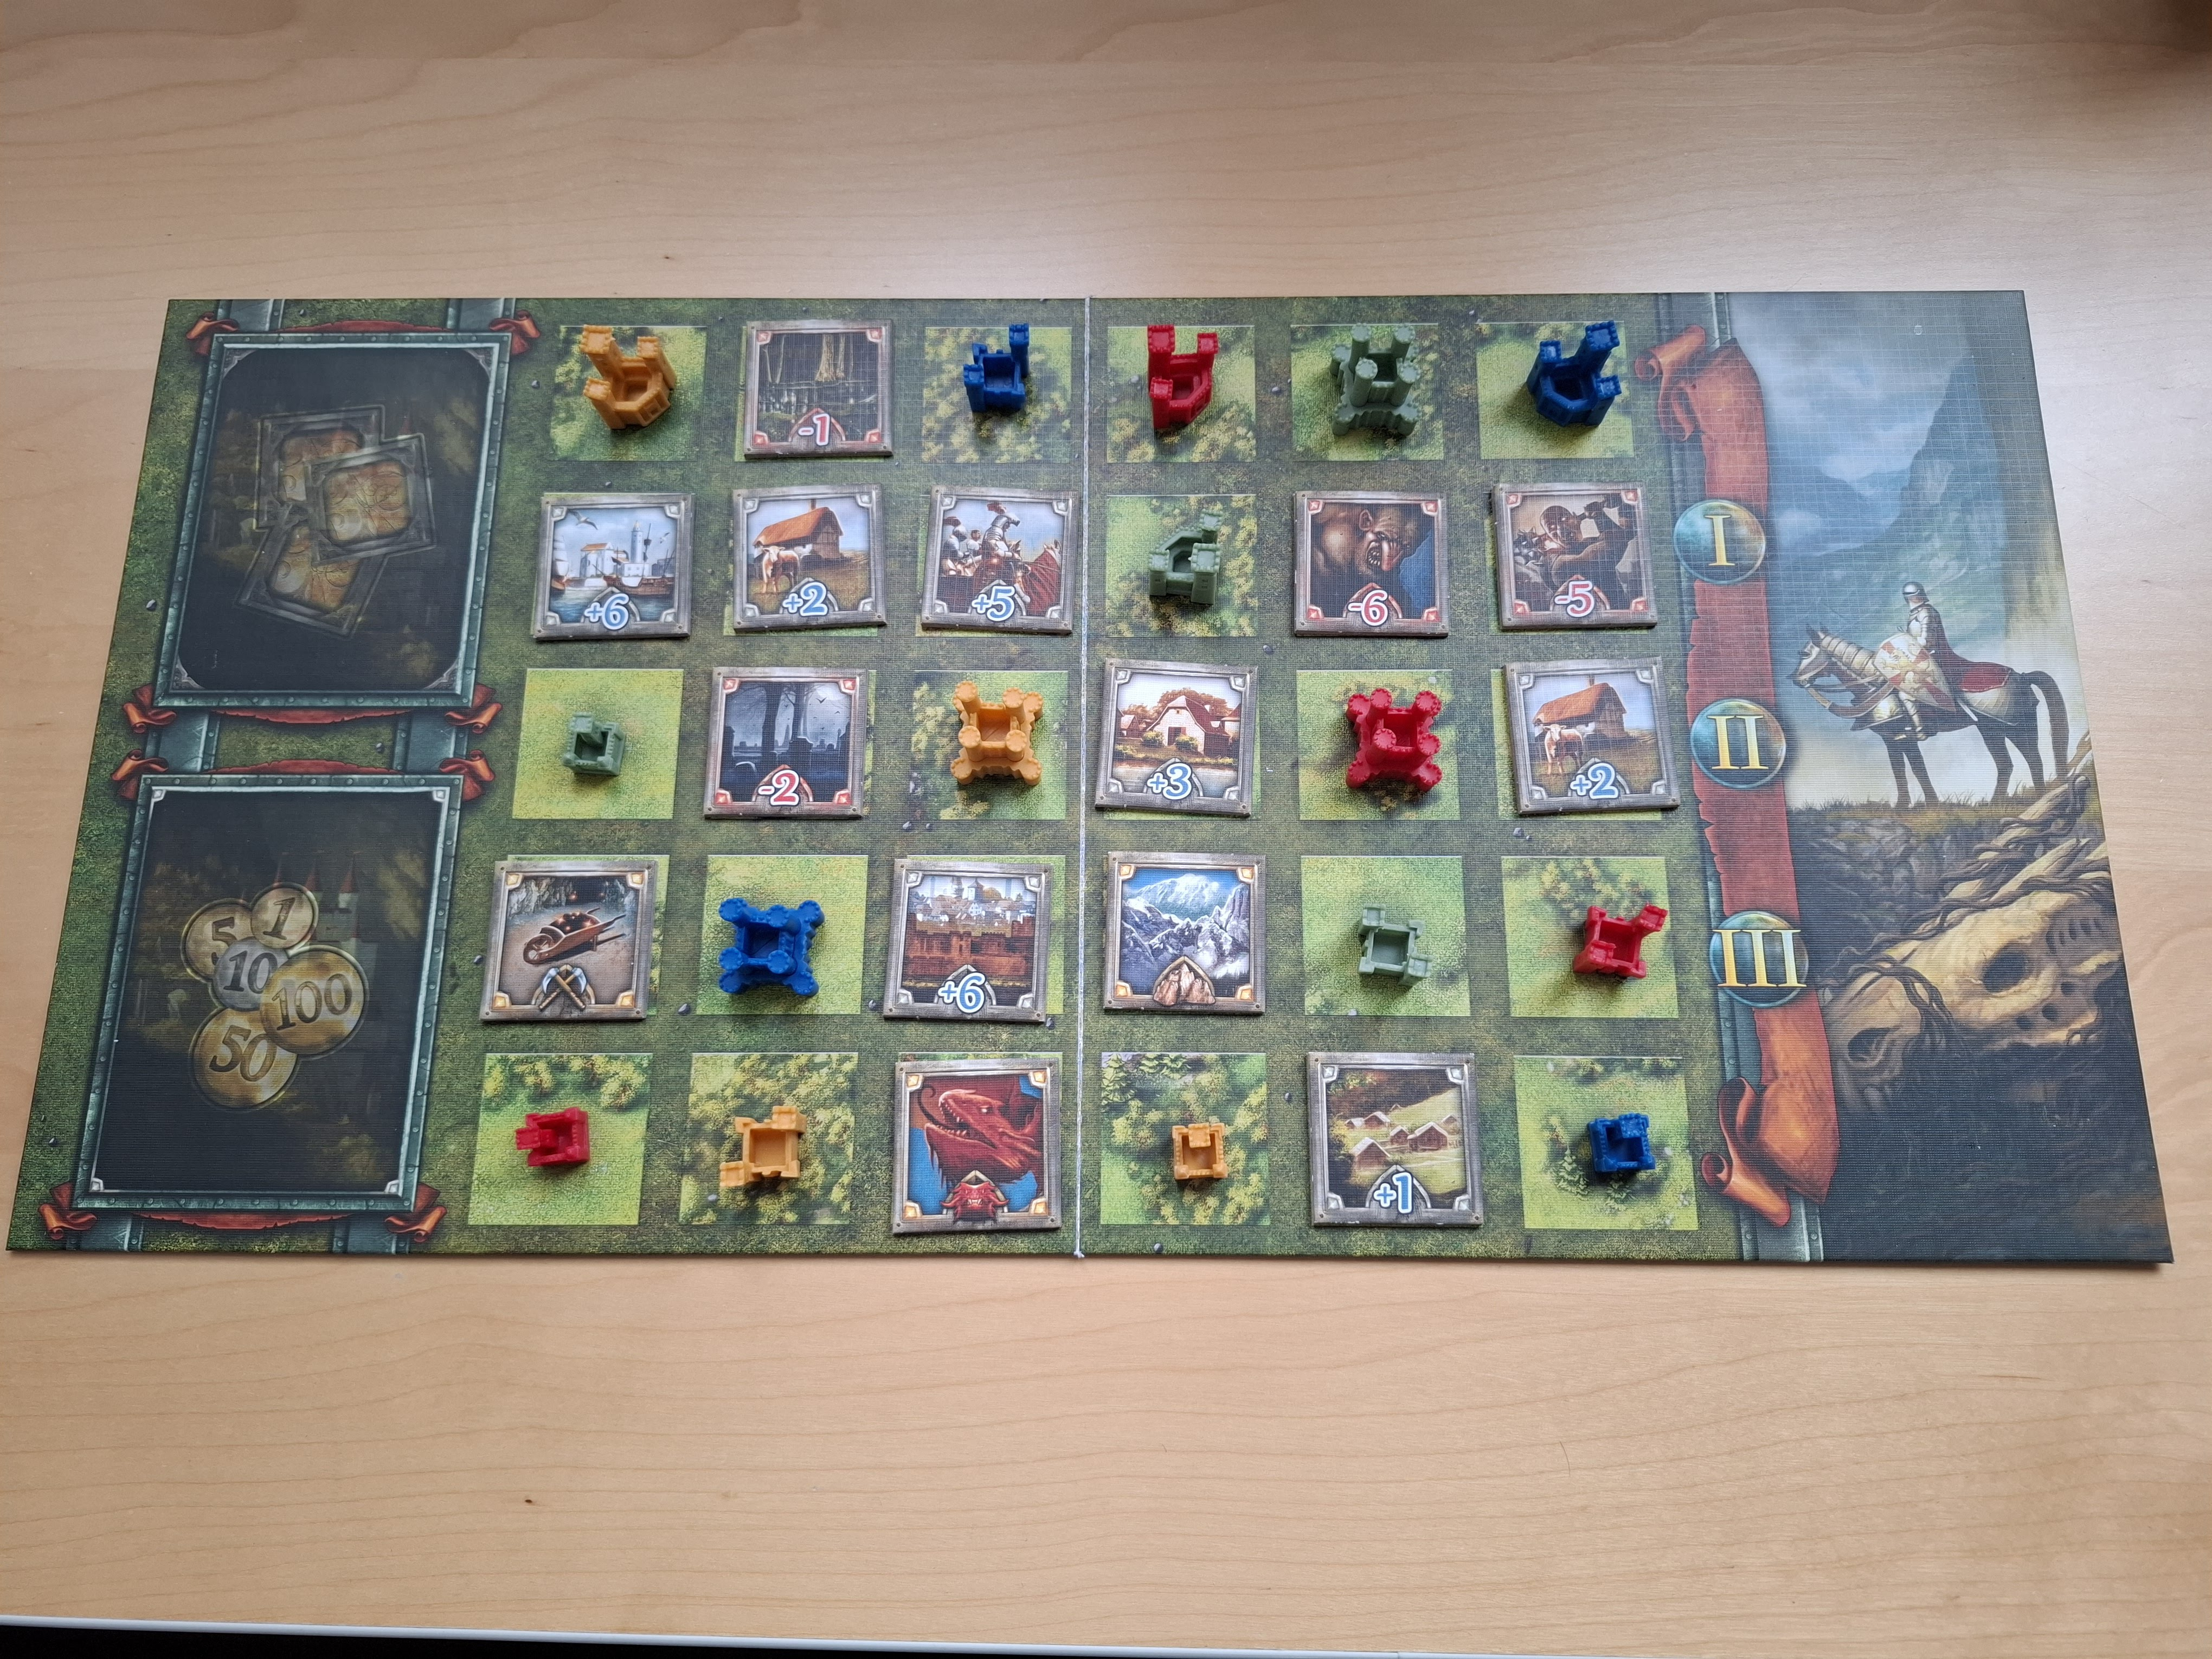
\includegraphics[width=1.0\linewidth]{figures/igraca_poca.jpg} 
		\caption{Primjer popunjene igraće ploče.}
		\label{slk:igraca_ploca}
	\end{figure}
	
	\section{Objekti na igraćoj ploči}
		Kao što je već spomenuto, elementi koje igrači mogu postaviti na ploču se mogu svrstati u dvije kategorije - dvorci i kartice. Dvorci pripadaju pojedinim igračima i njihova uloga je prikupljanje bodova. S druge strane postavljene kartice su dijeljeni elementi te mogu donositi pozitivne ili negativne bodove/resurse ili imati posebne efekte. Svi navedeni elementi igre koji se mogu postaviti na igraću ploču prikazani su na slici~\ref{slk:elementi_igre}
		
		\begin{figure}[htb]
			\centering
			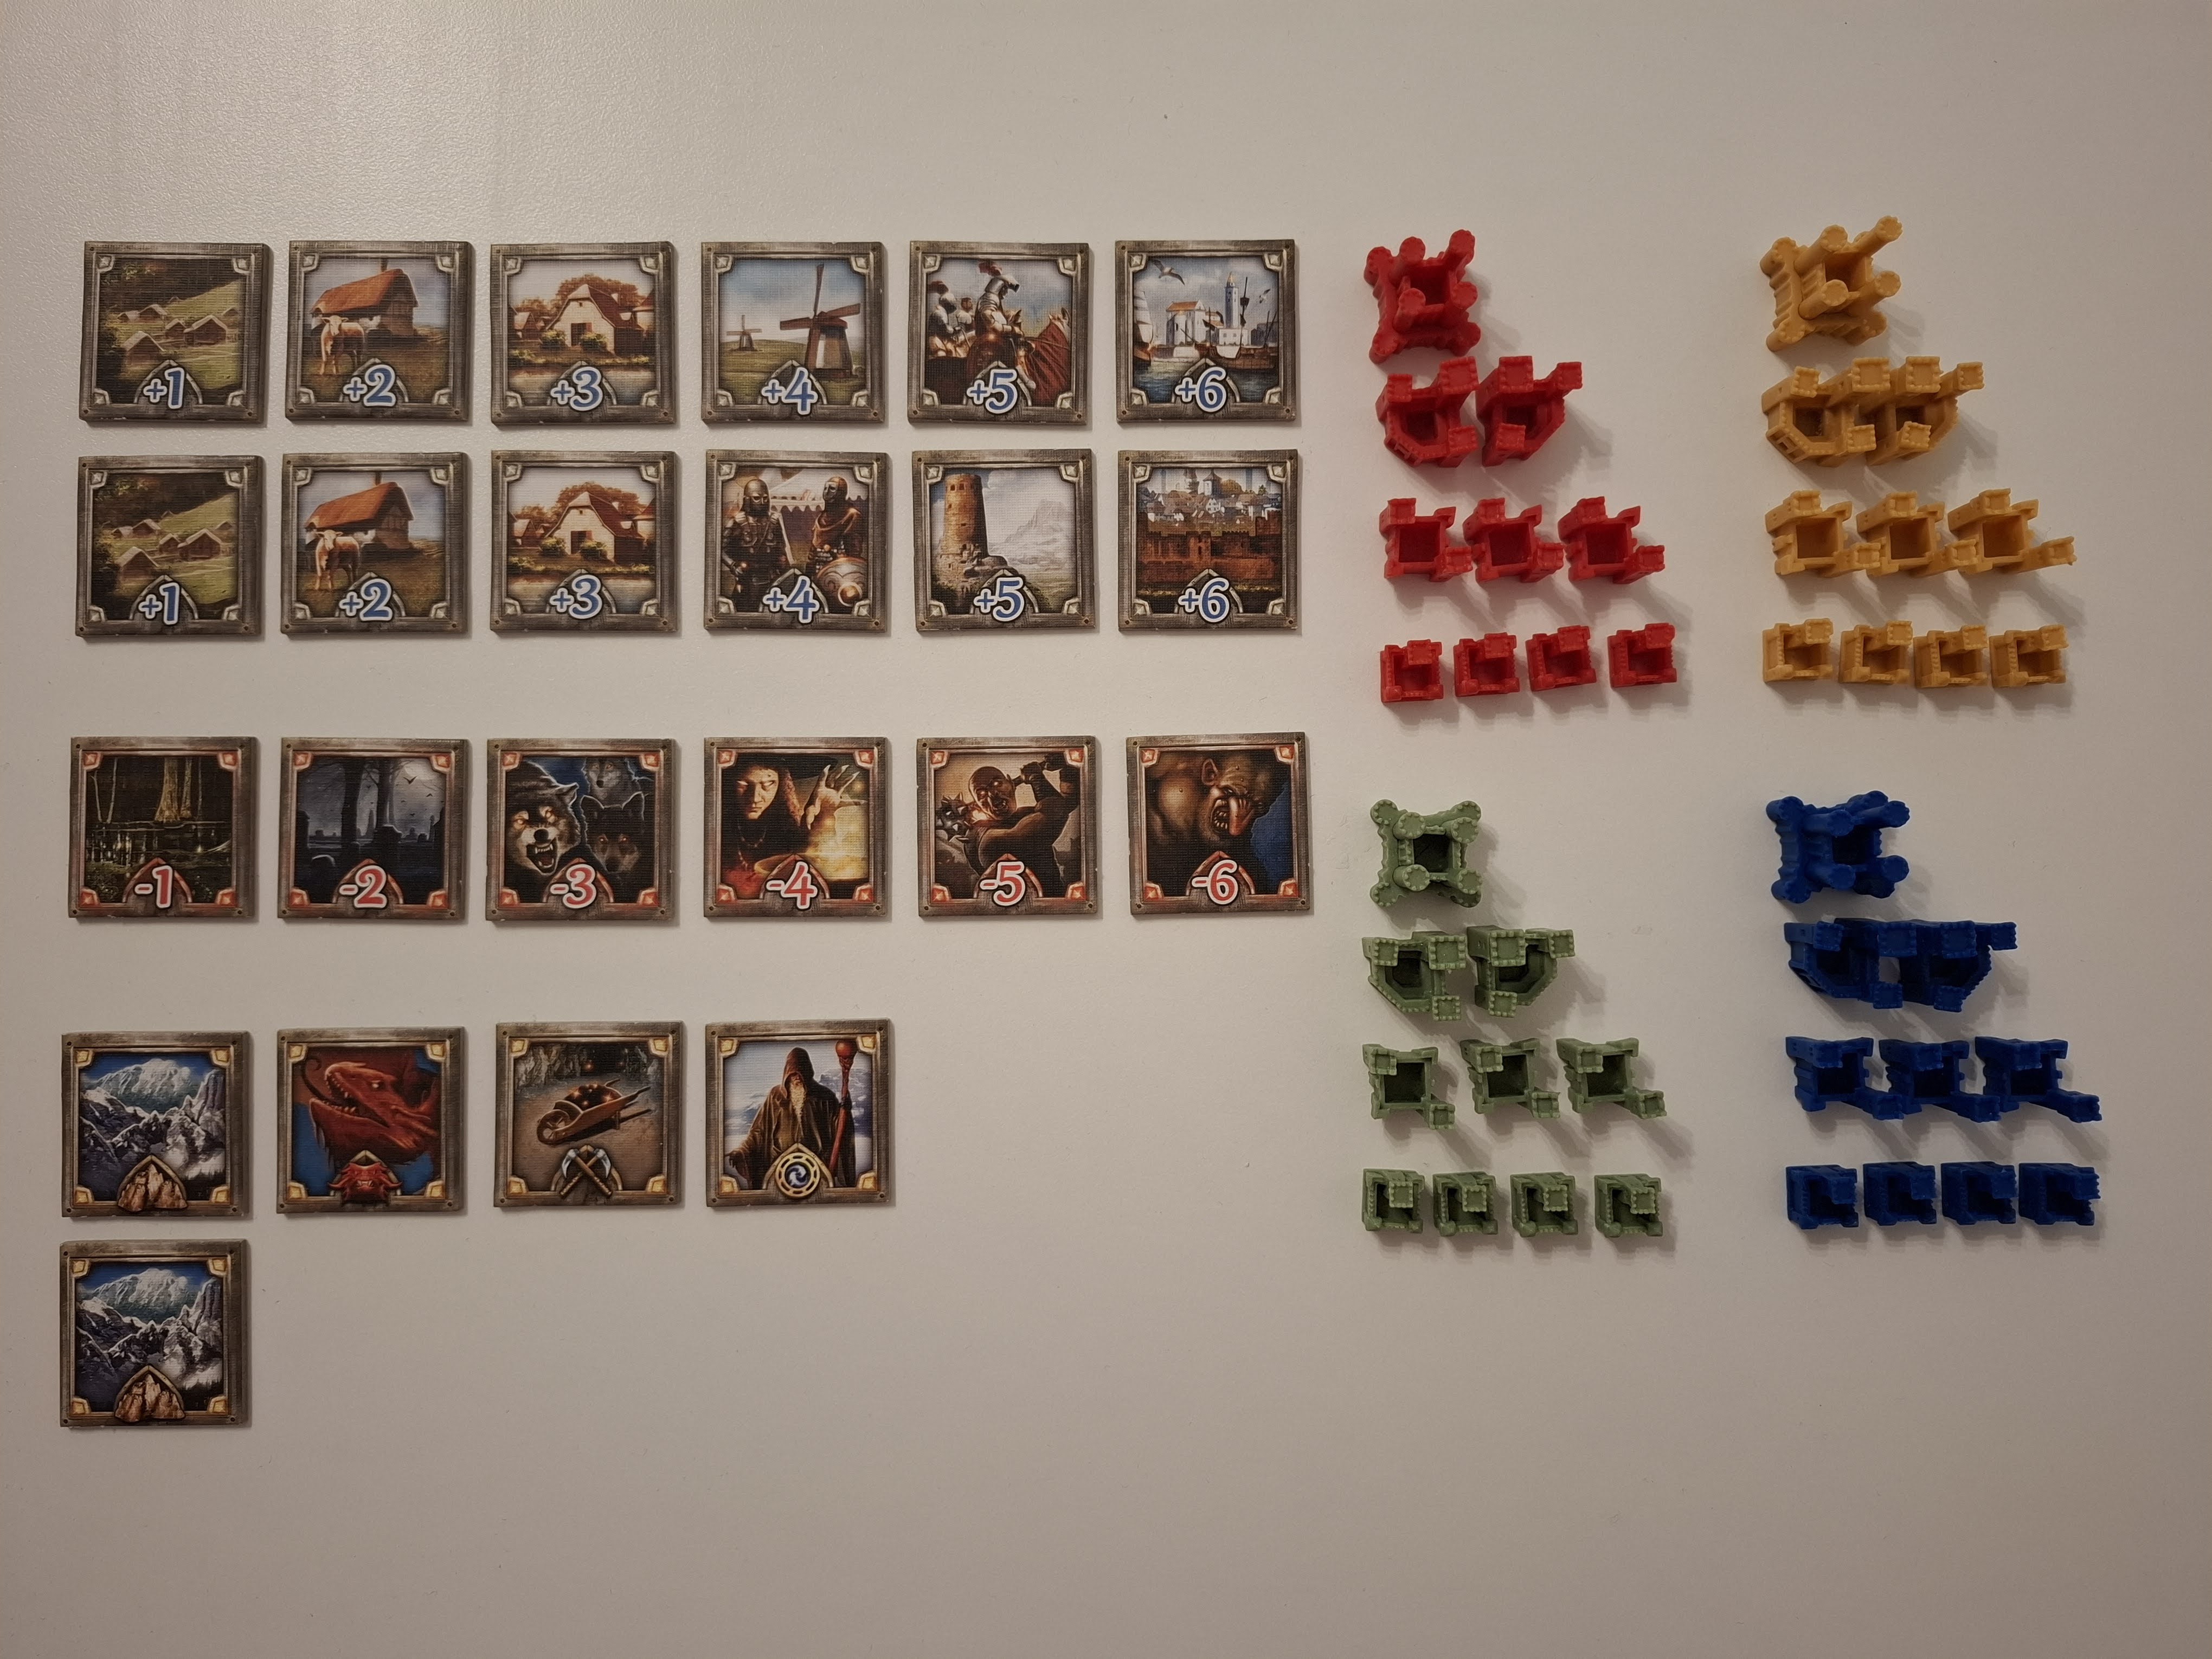
\includegraphics[width=1.0\linewidth]{figures/elementi_igre.jpg} 
			\caption{Kartice i dvorci igre.}
			\label{slk:elementi_igre}
		\end{figure}
		
		Dvorci dolaze u četiri boje, svaka za jednog igrača: crvena, zelena, plava i žuta. Dodatno, dvorci u svakoj boji se razlikuju po svojim razinama, odnosno rangovima. Svaka razina dvorca se prepoznaju po veličini i obliku dvorca. Tako u svakoj boji postoji četiri dvorca razine 1, tri dvorca razine 2, dva dvorca razine 3 i jedan dvorac razine 4. Dvorac prikuplja resurse u svojem retku i stupcu, a razina dvorca određuje multiplikator bodova koje je taj dvorac prikupio. Dvorci koji su iskorišteni u nekoj rundi se ne mogu ponovno koristiti u kasnijim rundama.
		
		Postoje dvije vrste kartica: kartice resursa i posebne kartice. Kartice resursa mogu donositi negativne ili pozitivne bodove, a bodovi su napisani na samim karticama. Pozitivne kartice donose bodove u iznosima od 1 do 6. Postoje dvije pozitivne kartice za svaku vrijednost bodova, dakle 12 kartica ukupno. Negativne kartice donose bodove u iznosima od -6 do -1 te postoji samo jedna kartica za svaku vrijednost negativnih bodova, dakle ukupno 6 kartica.
		
		Postoje 4 vrste specijalnih kartica: planina, zmaj, rudnik zlata i čarobnjak. Ove kartice ne donose bodove direktno, već utječu na druge kartice i dvorce u svojim redcima i stupcima. Kartica planine razdvaja redak i stupac u kojem se nalazi na dva dijela. Time efektivno taj redak i stupac postaju dva manja retka i stupca koja se promatraju odvojeno. Efekti s jedne strane planine nemaju utjecaj na drugoj strani planine. Postoje ukupno dvije takve kartice. Kartica zmaja poništava pozitivne kartice, ali samo za bodovanje retka i stupca u kojem se kartica zmaja nalazi. Postoji samo jedna takva kartica. Kartica rudnika zlata udvostručuje vrijednost svih kartica resursa, dakle i pozitivnih i negativnih. Taj efekt vrijedi samo tijekom bodovanja retka i stupca u kojem se nalazi kartica rudnika zlata. Postoji samo jedna kartica rudnika zlata. Kartica čarobnjaka uvećava rang svakog dvorca u svojem neposrednom 4-susjedstvu te postoji samo jedna takva kartica.
	
	\section{Pravila bodovanja}
		Runda završava kada se popune sva polja na ploči i tada počinje proces bodovanja. Prema službenim pravilima potrebno je bodovati svaki redak i stupac na ploči zasebno. Stupac/redak se boduje tako da se zbroje sve vrijednosti resursa u tom retku/stupcu, uključujući i pozitivne i negativne resurse. Nakon toga se za svaki dvorac na ploči zbrajaju bodovi retka i stupac u kojima se on nalazi te se ti bodovi množe s rangom dvorca. Dobiveni bodovi se dodjeljuju igraču kojemu dvorac pripada. Primjer kako se boduje konkretno stanje ploče je dostupan i u službenim pravilima~\cite{KingdomsRulebook}.

\chapter{Arhitektura sustava}
	\label{pog:arhitektura}
	
	Cijeli sustav je na vrlo visokoj razini apstrakcije opisan dijagramom prikazanim na slici~\ref{slk:arhitektura_sustava}. Sve počinje od fotografije igraće ploče koja je ulaz u sustav. Sustav prvo detektira ploču na fotografiji te detektiranu ploču ispravlja tako da neovisno o kutu iz kojeg je ploča uslikana uvijek dobivamo izrezanu ploču iz iste perspektive te u istim dimenzijama slike. Iz ispravljene slike ploče izrezuju se fotografije pojedinih pozicija u rešetki koja se nalazi na ploči. Ovaj dio sustava je ostvaren korištenjem klasičnih metoda računalnog vida, kao na primjer Cannyjev algoritam te Houghove transformacije.
	
	\begin{figure}[htb]
		\centering
		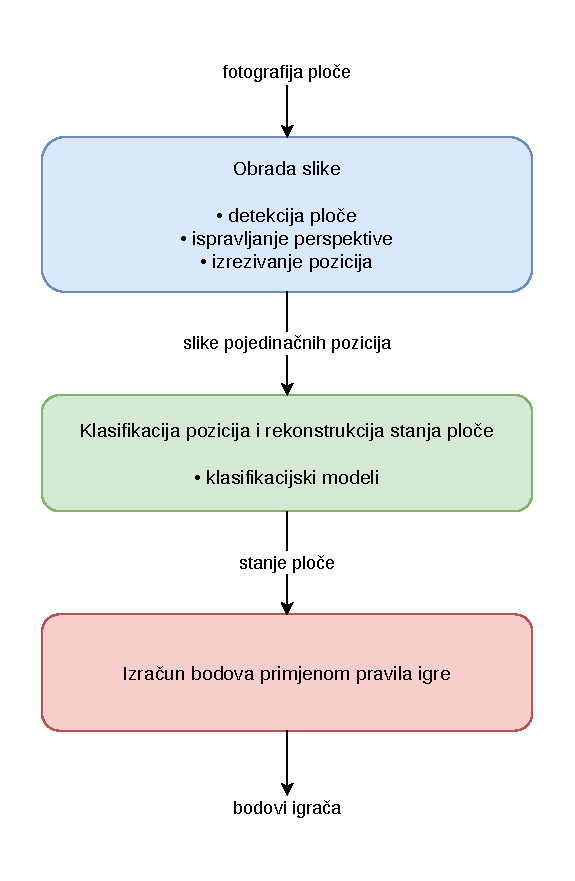
\includegraphics[width=0.64\linewidth]{figures/dijagram1.drawio.pdf} 
		\caption{Apstraktna arhitektura sustava za automatsko bodovanje.}
		\label{slk:arhitektura_sustava}
	\end{figure}
	
	Svaka pozicija je jedno polje koje sadrži neki objekt igre, bilo dvorac ili karticu. Izrezana polja ploče se trebaju analizirati kako bi se utvrdilo koji objekt se nalazi na konkretnom polju. U tu svrhu korištene su naprednije metode računalnog vida, konkretnije duboki konvolucijski modeli. S obzirom na to da se radi o metodama strojnog učenja, za ovakav pristup potreban je skup podataka za učenje. Tijekom pripremnog istraživanja i pripreme za izradu ovog rada nije pronađen niti jedan javno dostupan skup slika za učenje ove društvene igre. Zbog toga je u ovom radu dodatno izrađen vlastiti skup podataka za učenje. 
	
	S obzirom na ograničene resurse izrađen skup podataka za učenje je relativno skroman. Stoga je dodatno razvijen sustav za augmentaciju slika kojim se iz originalnih fotografija umjetno stvaraju nove vjerne varijacije originalne fotografije. Taj sustav je korišten tijekom treniranja dubokih modela kako bi se umjetno povećao skup podataka za treniranje.
	
	Na temelju prethodno opisane analize ulazne slike sustav izrađuje model stanja igre, to jest računalnu reprezentaciju ploče s njezinim sadržajem. Nad dobivenim modelom stanja igre jednostavno se primjenom pravila igre izračunavaju ostvareni bodovi za pojedinog igrača.
		
	\section{Detekcija ploče}
	\label{pog:detekcija}
		Problem detekcije ploče pojavljuje se na dva mjesta u procesu razvoja. Prvo mjesto je kod izrade skupa podataka za učenje, s obzirom na to da je potrebno iz generičkih fotografija ploče napraviti standardiziranu izrezanu fotografiju ploče iz perspektive direktnog pogleda odozgo. Drugo mjesto u kojem se pojavljuje detekcija ploče je u samoj mobilnoj aplikaciji kada korisnik uslika fotografiju. S obzirom na to da će modeli dubokog učenja kod korištenja aplikacije dobivati fotografije iz ovog procesa, bitno je da je i njihov skup podataka za učenje nastao iz identičnog procesa. Stoga je smisleno napraviti podsustav za detekciju koji će se dijeliti u oba procesa. Ovaj podsustav je odabran prvi za razvoj jer je izrada skupa podataka za učenje osnovni preduvjet za daljnji razvoj dubokih modela.
		
		Ovaj proces se može podijeliti na tri dijela opisana dijagramom na slici~\ref{slk:arhitektura_detekcije}. Prvo se traži četverokutna kontura ploče na originalnoj slici. Na temelju dobivene konture dobivaju se točke uglova ploče. Točke uglova se dalje koriste kod ispravljanja slike tako da se dobije standardizirana slika ploče. Na kraju se na standardiziranu sliku primjenjuje fiksna rešetka na temelju koje se izrezuju pojedinačna polja s ploče. Dobivene izrezane fotografije se koriste u daljnjim koracima.
		
		\begin{figure}[htb]
			\centering
			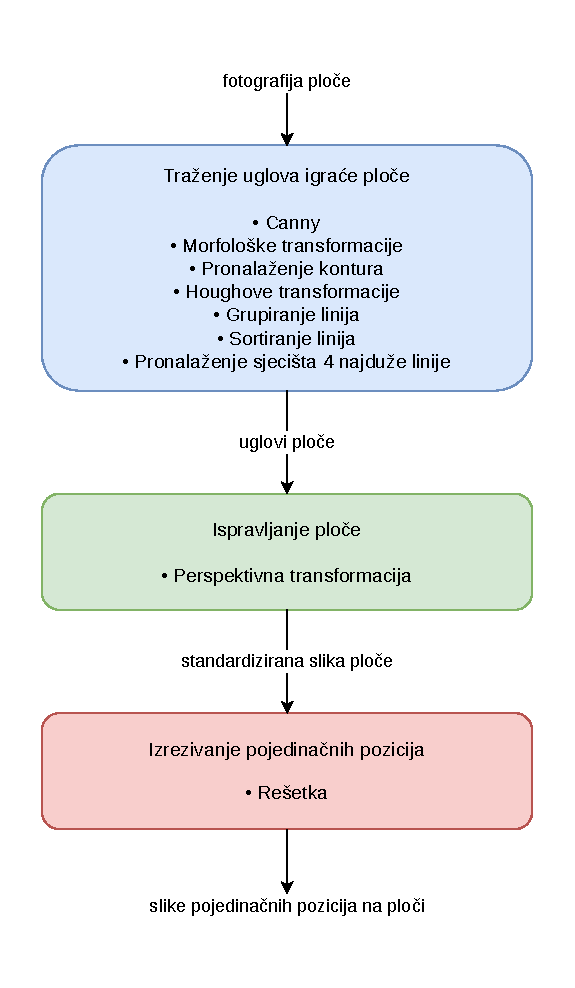
\includegraphics[width=0.64\linewidth]{figures/dijagram2.drawio.pdf} 
			\caption{Apstraktna arhitektura sustava detekciju ploče i izrezivanje pozicija.}
			\label{slk:arhitektura_detekcije}
		\end{figure}

		\subsection{Traženje uglova ploče}
			Prvi korak u traženju uglova ploče je pretprocesiranje. Slika se prvo skalira tako da najveća dimenzija slike iznosi 1000 piksela. Nakon toga slijedi transformacija slike u sivi spektar. Završno se primjenjuje relativno jako Gaussovo zamućenje kako bi se uklonio šum i sitni detalji. 
			
			Sada slijedi procesiranje slike. Prvi korak ovdje je primjena Cannyjevog algoritma za detekciju linija uz dosta niske i tolerantne pragove. Rezultat ovog algoritma je binarna slika u kojoj pikseli s vrijednosti 1 (u skali 0-1). Primjer detektiranih linija pomoću Cannyjevog algoritma je vidljiv na slici~\ref{slk:canny}.
			
			% \textit{SLIKA IZLAZ CANNYJA}
			\begin{figure}[htb]
				\centering
				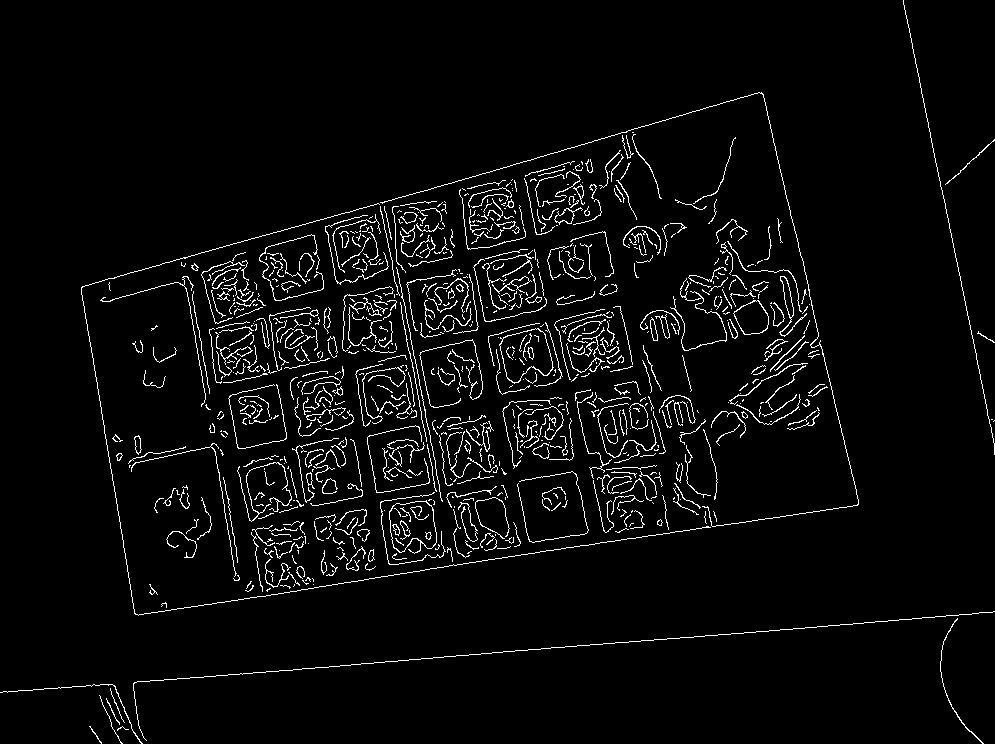
\includegraphics[width=1.0\linewidth]{figures/canny.png} 
				\caption{Rezultat Cannyjevog algoritma detekcije linija.}
				\label{slk:canny}
			\end{figure}
			
			Kako bi se zatvorili potencijalni prekidi u detektiranim linijama, sljedeće se provodi morfološka transformacija zatvaranja. Općenito, morfološke operacije rade nad binarnim slikama te su slične konvoluciji u smislu da se koriste male jezgre kojima se prolazi kroz sliku~\cite{MorphologicalOperations}. Dvije osnovne morfološke transformacije su erozija i dilatacija~\cite{MorphologicalOperations}. Kod erozije će piksel u originalnoj slici biti postavljen na 1 samo ako svi pikseli u originalnoj slici pokriveni jezgrom također imaju vrijednost 1~\cite{MorphologicalOperations}. Kod dilatacije se pak piksel u originalnoj slici postavlja na 1 ako je barem jedan piksel u originalnoj slici pokriven jezgrom ima vrijednost 1. Morfološko zatvaranje je kombinacija dilatacije nakon koje slijedi erozija~\cite{MorphologicalOperations}. Ovom transformacijom se dakle postiže zatvaranje malih prekida u linijama koje je detektirao Cannyjev algoritam. Rezultat ove transformacije nad detektiranim linijama sa slike~\ref{slk:canny} je vidljiv na slici~\ref{slk:morfoloske_transformacije}.
			
			\begin{figure}[htb]
				\centering
				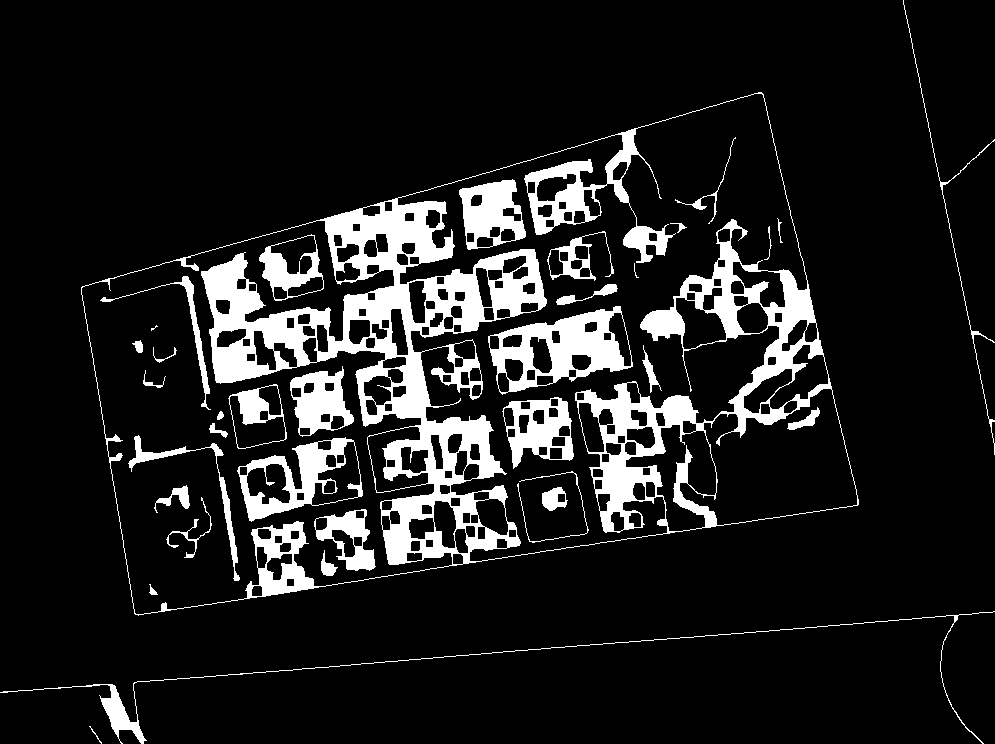
\includegraphics[width=1.0\linewidth]{figures/morfoloske_transformacije.png} 
				\caption{Rezultat morfološke transformacije zatvaranja.}
				\label{slk:morfoloske_transformacije}
			\end{figure}
			
			Slijedi pronalaženje kontura na rezultantnoj slici. Konture se pronalaze pomoću algoritma kojeg su objavili Suzuki i Abe~\cite{SUZUKI198532}. Radi se o algoritmu praćenja granice koji prati hijerarhiju kontura. Dodatno, korištena je varijanta koja gleda samo vanjske konture. To znači da ako postoji kontura koja je u potpunosti sadržana u većoj vanjskoj konturi, onda se ta unutarnja kontura ne gleda~\cite{SUZUKI198532}.
			
			Nakon toga se dobiven konture sortiraju te se uzima kontura najveće površine. Objašnjenje za ovo je sljedeće: ako analiziramo sliku igraće ploče, onda je razumno za pretpostaviti da će ploča dominirati u fotografiji, to jest da će biti objekt s najvećom konturom na slici. Najveća pronađena kontura na slici~\ref{slk:morfoloske_transformacije} je prikazana na slici~\ref{slk:kontura}.
			
			\begin{figure}[htb]
				\centering
				
\includegraphics[width=1.0\linewidth]{figures/kontura.png} 
				\caption{Najveća pronađena kontura.}
				\label{slk:kontura}
			\end{figure}
			
			Sljedeći korak je pronalaženje ravnih linijskih segmenata na najvećoj konturi pomoću Houghovih transformacija. Konkretno, koristi se progresivne probabilističke Houghove transformacije kojeg je objavio Matas sa suradnicima~\cite{ProgressiveProbabilisticHough}. Ukratko, radi se o varijaciji standardne Houghove transformacije koja koristi uzorkovane točke linija~\cite{ProgressiveProbabilisticHough}. Dodatno, ova varijacija može odrediti ravne linije tijekom glasanja točaka. Ako se tako odredi nova ravna linija, točke koje joj pripadaju se izbacuju te se tako proces računski ubrzava~\cite{ProgressiveProbabilisticHough}.
			
			\begin{figure}[htb]
				\centering
				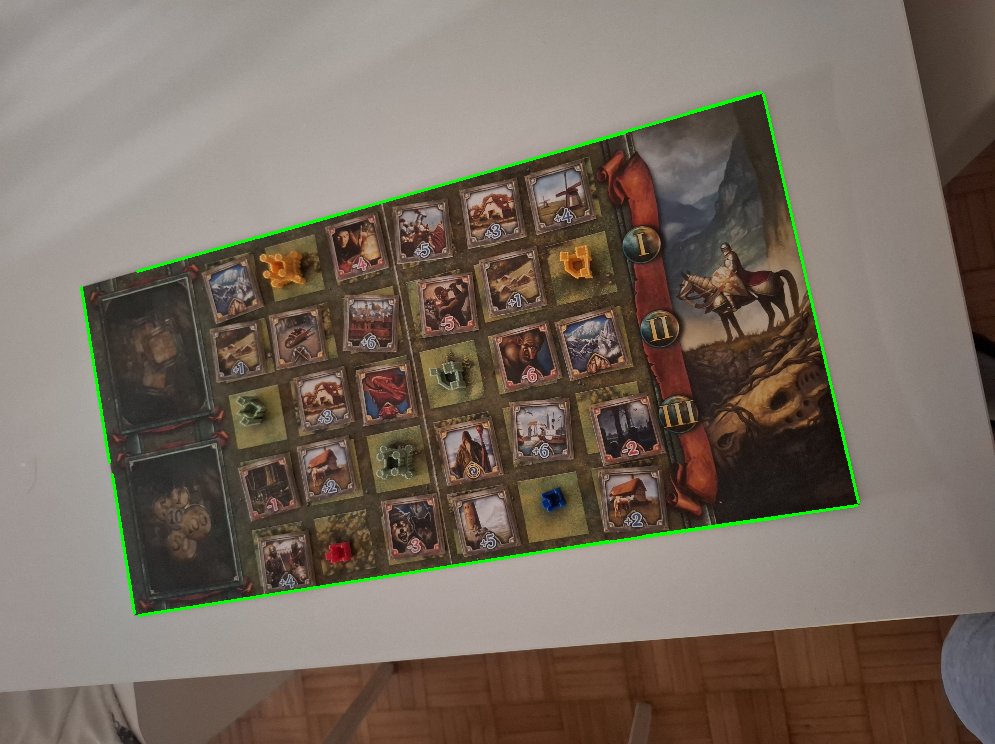
\includegraphics[width=1.0\linewidth]{figures/Hough.png} 
				\caption{Linije dobivene Houghovom transformacijom.}
				\label{slk:hough_og}
			\end{figure}
			
			Dobiveni rezultat na primjeru slike~\ref{slk:kontura} je vidljiv na slici~\ref{slk:hough_og}. Rezultantni skup ravnih linija je često dosta šumovit. Događa se da se oko stvarne linije sa slike pronalazi puno linija koje često nisu nužno na istom pravcu, ali su paralelne ili skoro paralelne. Zbog toga je sljedeće napravljeno jednostavno grupiranje linija. 
			
			Grupiranje je izvršeno prema parametrima linija dobivenih iz Houghove transformacije, dakle udaljenost pravca od ishodišta koordinatnog sustava i kut pravca. Na početku grupiranja postoji prazna lista grupa. Algoritam iterira po linijskim segmentima te svaki linijski segment pridružuje prvoj grupi kojoj su udaljenosti oba parametra od parametara linijskog segmenta unutar definiranih pragova. Ako se linijski segment nije mogao pridružiti niti jednoj grupi, onda se za njega stvara nova grupa. Prilikom svakog pridruživanja linijskog segmenta ažuriraju se parametri pripadne grupe kao aritmetička sredina parametara svih linija koje čine grupu. Algoritam grupiranja završava prolaskom kroz sve linijske segmente.
			
			Iz dobivenih grupa konstruirani su novi linijski segmenti tako da se za orijentaciju novog segmenta uzima orijentacija pripadne grupe, a kao krajnje toče se uzimaju najekstremnije točke od svih linijskih segmenata u toj grupi. Ideja za ovakav pristup je da se kombiniranjem više kraćih sličnih linija složi nova dugačka linija koja će pratiti prepoznatu liniju iz originalne slike po većem području, što će biti bitno kasnije.
			
			Nakon toga je provedeno još jedno grupiranje novonastalih linijskih segmenata po istom principu, ali uz veću toleranciju na dopušteno odstupanje parametara segmenta od parametara grupe. Ovog puta se kod nastalih grupa zadržava samo najduži linijski segment iz svake grupe kako bi se dodatno izbacile šumovite linije. Primjer preostalih linija nakon ovih grupiranja je prikazan na slici~\ref{slk:hough_konacan}. 
			
			\begin{figure}[htb]
				\centering
				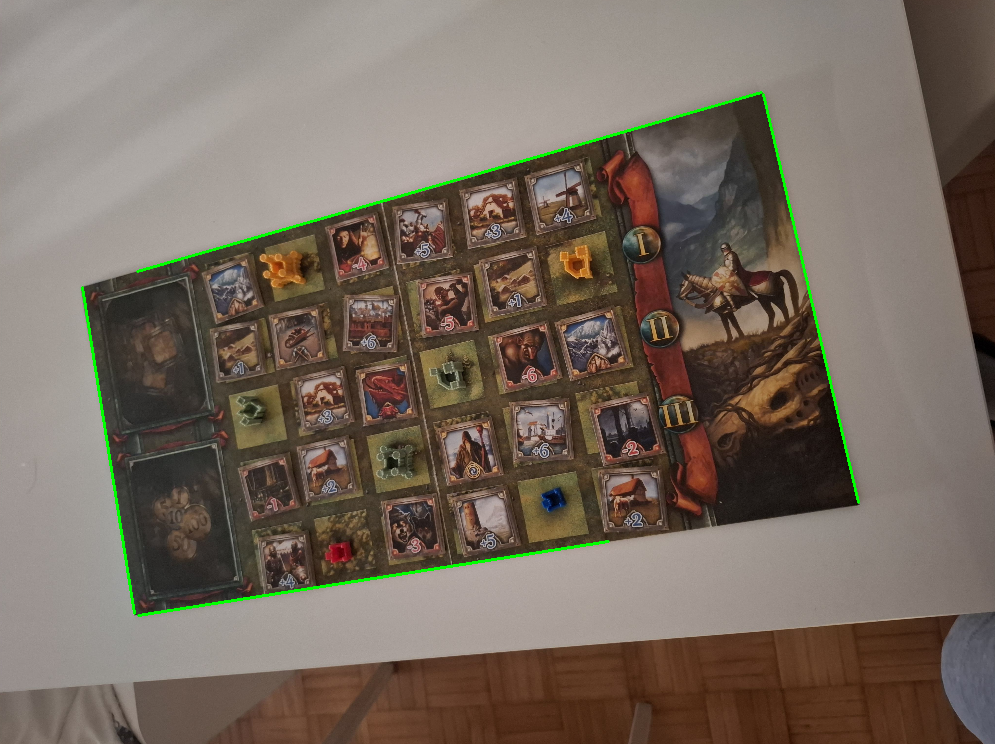
\includegraphics[width=1.0\linewidth]{figures/Hough_clustered.png} 
				\caption{Detektirane linije nakon grupiranja.}
				\label{slk:hough_konacan}
			\end{figure}
			
			Sljedeći korak se ponovno vodi pretpostavkom da će igraća ploča dominirati na originalnoj slici te da će dominantne linije na slici zbog toga pripadati upravo toj ploči. Zato na kraju provodi sortiranje preostalih linija te se uzimaju četiri najduže linije. Za njih se pretpostavlja da su upravo rubovi ploče. Na primjeru slike~\ref{slk:hough_konacan} već je preostalo samo četiri linija, ali to nije slučaj u svakom primjeru. 
			
			Posljednji korak je pronalaženje sjecišta dobivenih linija. Dobivena sjecišta su uglovi ploče, a oni su potrebni za sljedeći korak ispravljanja slike. Pronađeni uglovi na temelju četiri najdulje linije sa slike~\ref{slk:hough_konacan} su prikazani na slici~\ref{slk:uglovi}.
			
			\begin{figure}[htb]
				\centering
				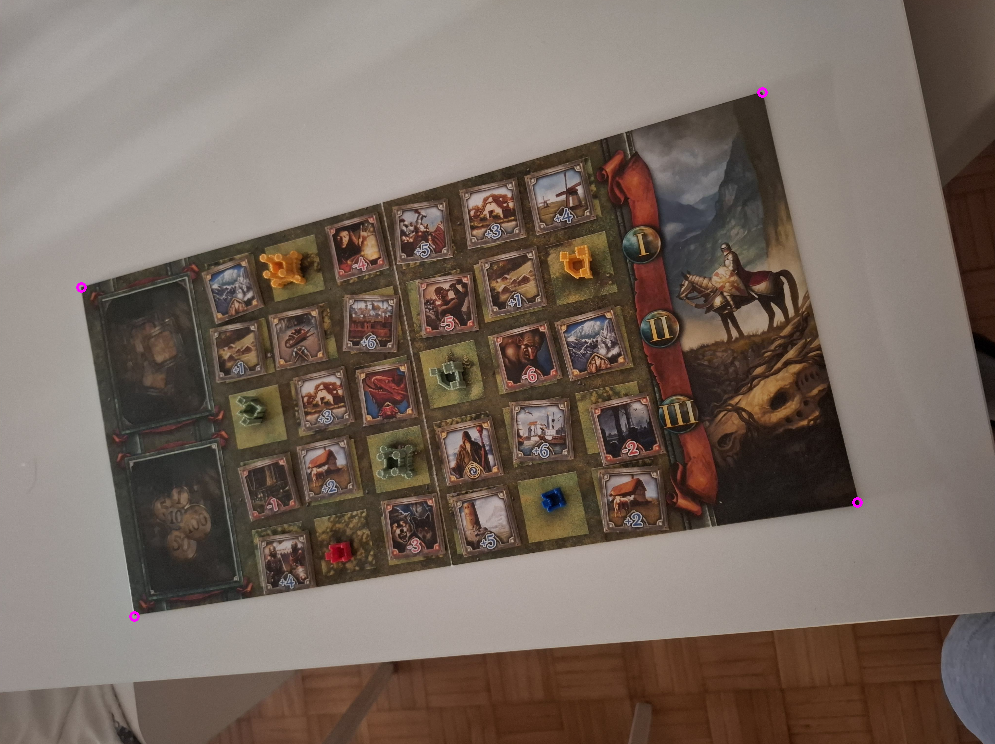
\includegraphics[width=1.0\linewidth]{figures/uglovi.png} 
				\caption{Pronađeni uglovi ploče.}
				\label{slk:uglovi}
			\end{figure}
		
		\subsection{Ispravljanje ploče}
			% citirati racvid prezentaciju?
			Cilj ispravljanja originalne slike ploče je dobiti sliku sa standardiziranom perspektivom na kojoj igraća ploča zauzima sav prostor, to jest da se vrhovi ploče nalaze upravo u vrhovima slike. Ovo se dobiva jednostavnom perspektivnom transformacijom. Za to nam je potrebno 4 korespondentnih točaka na originalnoj i ciljanoj slici. Upravo zato je bilo potrebno odrediti kutove ploče - to su korespondentne točke u originalno slici. U ciljanoj slici želimo točke uglova ploče preslikati u vrhove slike, a ciljana slika će uvijek biti fiksnih dimenzija pa su točke u ciljanoj slici također poznate. Iz danih korespondencija određuje se matrica perspektivne transformacije te se s pomoću nje provodi sama transformacija. Rezultat perspektivne transformacije na primjeru slike~\ref{slk:uglovi} s pronađenim uglovima je vidljiv na slici~\ref{slk:ispravljena_ploca}.
			
			\begin{figure}[htb]
				\centering
				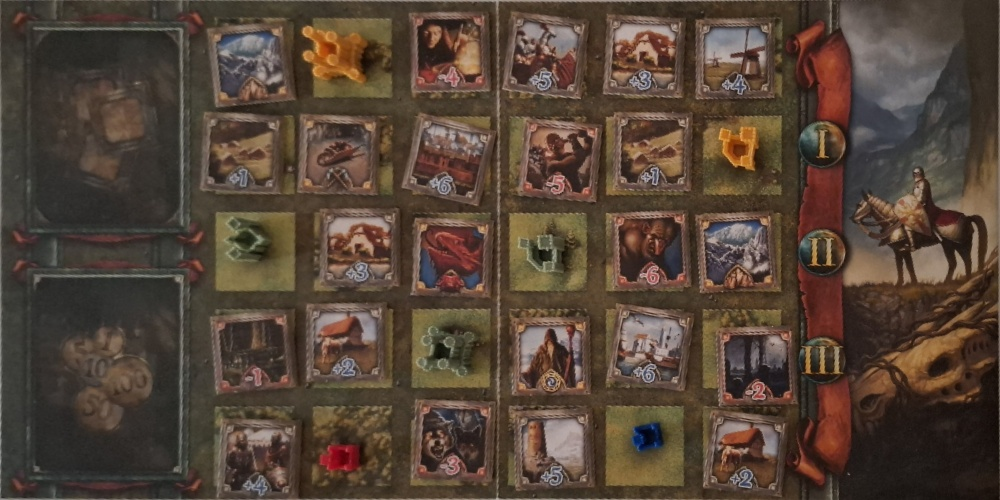
\includegraphics[width=1.0\linewidth]{figures/ispravljena_ploca.jpg} 
				\caption{Rezultat perspektivne transformacije.}
				\label{slk:ispravljena_ploca}
			\end{figure}
		
		\subsection{Izrezivanje polja}
			Kada je dobivena standardizirana ispravljena slika ploče potrebno je još samo izrezati pojedina polja na ploči. Ovdje problem značajno olakšava činjenica da je rešetka s poljima postavljena na sredinu ploče te je potpuno simetrična. Zbog toga je za ovaj dio problema bilo dovoljno koristiti fiksnu rešetku pomoću koje su izrezivana pojedinačna polja ploče. Dimenzije pojedinog polja na korištenoj rešetci su podešene tako da najbolje odgovaraju stvarnoj rešetki na igraćoj ploči.
			
			Ovakav pristup ne radi savršeno zbog malih odstupanja kod detekcije kutova ploče koji se mogu dogoditi, ali je dovoljno dobar za potrebe ovog projekta. S obzirom na spomenutu nesavršenost rešetke te činjenice da elementi postavljeni na pojedinim poljima mogu biti pomaknuti s točne pozicije postoji opasnost da ciljani objekt na danoj poziciji ne bude u potpunosti obuhvaćen prilikom izrezivanja. Zbog toga se koristi dodatna margina tako da se prilikom izrezivanja dodatno uzima i širi prostor oko same pozicije tako da ciljani objekt bude dobro obuhvaćen. Primjer primijenjene rešetke nad ispravljenom slikom~\ref{slk:ispravljena_ploca} je prikazan na slici~\ref{slk:resetka}.
			
			\begin{figure}[htb]
				\centering
				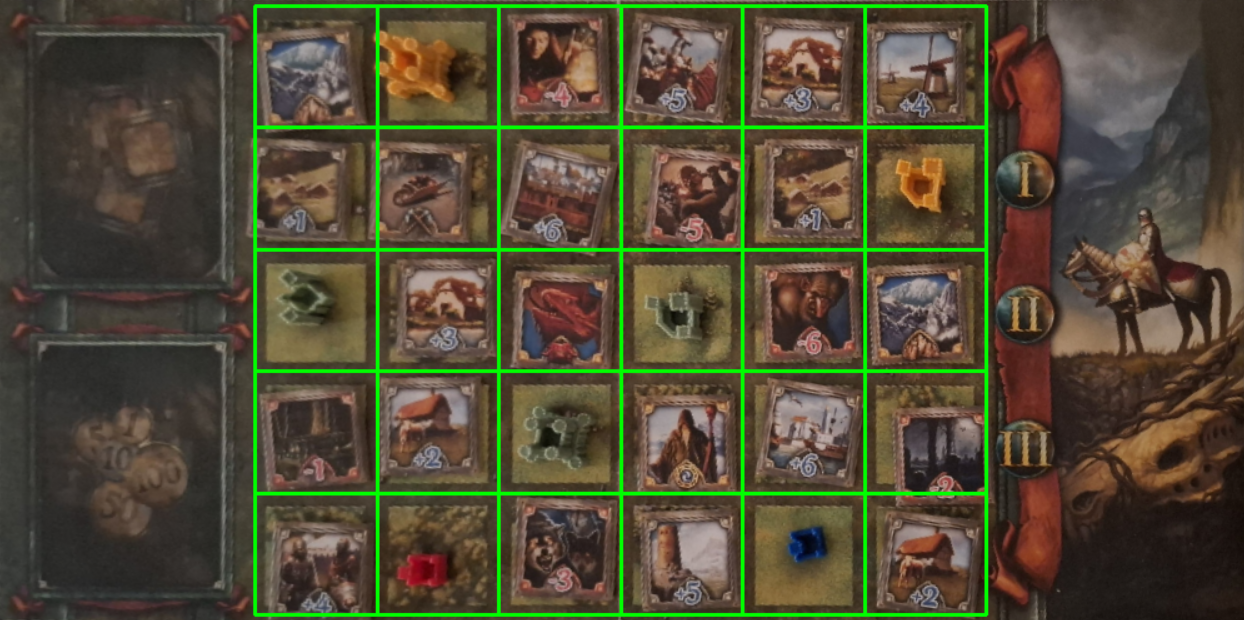
\includegraphics[width=1.0\linewidth]{figures/resetka.png} 
				\caption{Rešetka primijenjena na ispravljenu sliku ploče.}
				\label{slk:resetka}
			\end{figure}
		
	\section{Stvaranje skupa podataka za učenje}
		Kao što je ranije rečeno, potrebno je izraditi skup podataka za učenje dubokih modela koje će sustav koristiti. Duboki modeli će klasificirati sličice pojedinačnih objekata na ploči. Sličice će se dobivati postupkom opisanim u poglavlju \ref{pog:detekcija}. Skup podataka za učenje će se zbog toga sastojati od sličica pojedinačnih polja na rešetki ploče koja će sadržavati elemente igre (dvorce i kartice).
		
		U tu svrhu napravljene su fotografije igraće ploče u raznim konfiguracijama i uvjetima. Ploča je fotografirana u uvjetima slabog i dobrog osvjetljenja, uz prirodno osvjetljenje, osvjetljenje sobe te svijetlo stolne svjetiljke. Također je napravljeno nekoliko fotografija ploče u uvjetima jako izraženih sjena u vrijeme zalaska sunca. Fotografije su uslikane odozgo uz umjerene varijacije kuta i perspektive.
		
		Isprobavane su razne konfiguracije elemenata igre na ploči. Dodatno, fotografirane su i ploče na kojima se nalaze prazna polja tako da skup podataka sadrži i dodatnu klasu praznog polja. Iako prema pravilima igre na kraju svake runde ne mogu postojati prazna polja, ova klasa je uvedena radi potpunosti i robusnosti sustava. Ovime je također omogućeno da korisnik konačne aplikacije može fotografirati ploču i prije završetka runde za analizu trenutačnog stanja usred trajanja runde.
		
		Fotografije ploče su bile provučene kroz prethodno opisan sustav za detekciju ploče i izrezivanje pojedinih polja. Dobivene slike izrezanih polja su zatim spremljene te one predstavljaju same podatke za učenje.
		
		Fotografije ploča su dodatno korištene za evaluaciju samog sustava za detekciju ploče. U tu svrhu, sama ploča je fotografirana na 3 različite podloge: bijeli stol, crni stol te stol teksture svijetlog drva. Na taj načine se evaluiralo kako se detekcija ponaša uz različite kontraste pozadine i ploče. Sustav je uspješno detektirao ploču na svim fotografijama, kojih je bilo 57, na svim pozadinama te uvjetima osvjetljenja i sjena.
	
		\subsection{Označavanje podataka} % ili u privitak?
			\label{podpog:oznacanjavnje}
			Ovdje se radi o problemu nadziranog učenja što znači da podaci moraju imati svoje oznake. Međutim, u ovom konkretnom slučaju klasifikacija se radi u više koraka pomoću više modela, što je detaljnije objašnjeno u poglavlju~\ref{pog:klasifikacija}. Različiti modeli za iste podatke trebaju različite oznake. Na primjer, jedan model za svaku sliku donosi klasifikacijsku odluku radi li se o praznom polju, polju s karticom ili polju s dvorcem. Za taj model postoje oznake \textit{empty}, \textit{card} i \textit{castle}. Neki drugi model klasificira dvorce prema njihovom rangu te takav model koristi oznake \textit{1}, \textit{2}, \textit{3} i \textit{4}.
			
			Dakle, u ovom skupu podataka podaci imaju složene oznake koje sadržavaju potpunu informaciju o svakoj slici.Takva složena oznaka se sastoji od više oznaka koje se mogu koristiti ovisno o konkretnom problemu. Svaka složena oznaka prvo sadrži oznaku o vrsti objekta na slici koja definira radi li se o slici praznog polja, polja s karticom ili polja s dvorcem (pripadne oznake \textit{empty}, \textit{card} i \textit{castle}). 
			
			Ako se radi o slici kartice, slijedi oznaka o vrsti kartice, to jest radi li se o kratici s brojevnom vrijednosti ili posebnoj kartici (oznake \textit{number} i \textit{special}). Ako se radi o kartici s brojevnom vrijednosti slijedi oznaka koja je jednaka vrijednosti na kratici (oznake od \textit{-6} do \textit{-1} te od \textit{1} do \textit{6}). U suprotnom slijedi oznaka konkretne posebne kartice (oznake \textit{dragon}, \textit{gold mine}, \textit{mountain} i \textit{wizard}).
			
			Ako pak prva oznaka označava da se radi o slici dvorca, slijede dvije oznake koje opisuju boju i rang dvorca. Oznake boje dvorca su \textit{red}, \textit{green}, \textit{blue} i \textit{yellow}. Oznake za rang dvorca su \textit{1}, \textit{2}, \textit{3} i \textit{4}.
			
			Kako bi se ubrzao proces označavanja podataka dodatno je napravljena jednostavna aplikacija za označavanje slika. Sučelje aplikacije je vidljivo na slici~\ref{slk:oznacavanje}. Aplikacija omogućuje pregled neoznačenih slika i dodjeljivanje njihovih složenih oznaka. Također je omogućen i pregled već označenih slika te izmjena njihovih oznaka. Oznake se mogu dodijeliti ili izmijeniti korištenjem gumbova kojima se efektivno opisuje sadržaj slike. Postupak označavanja gumbovima prati prethodno opisanu strukturu složene oznake. Oznake se dodatno mogu dodijeliti ili izmijeniti korištenjem tipkovničkih prečaca. Tako se pritiskom jedne ili kombinacijom dvije tipke na tipkovnici može dodijeliti potpuna oznaka što uvelike ubrzava proces označavanja.
		
			\begin{figure}[htb]
				\centering
				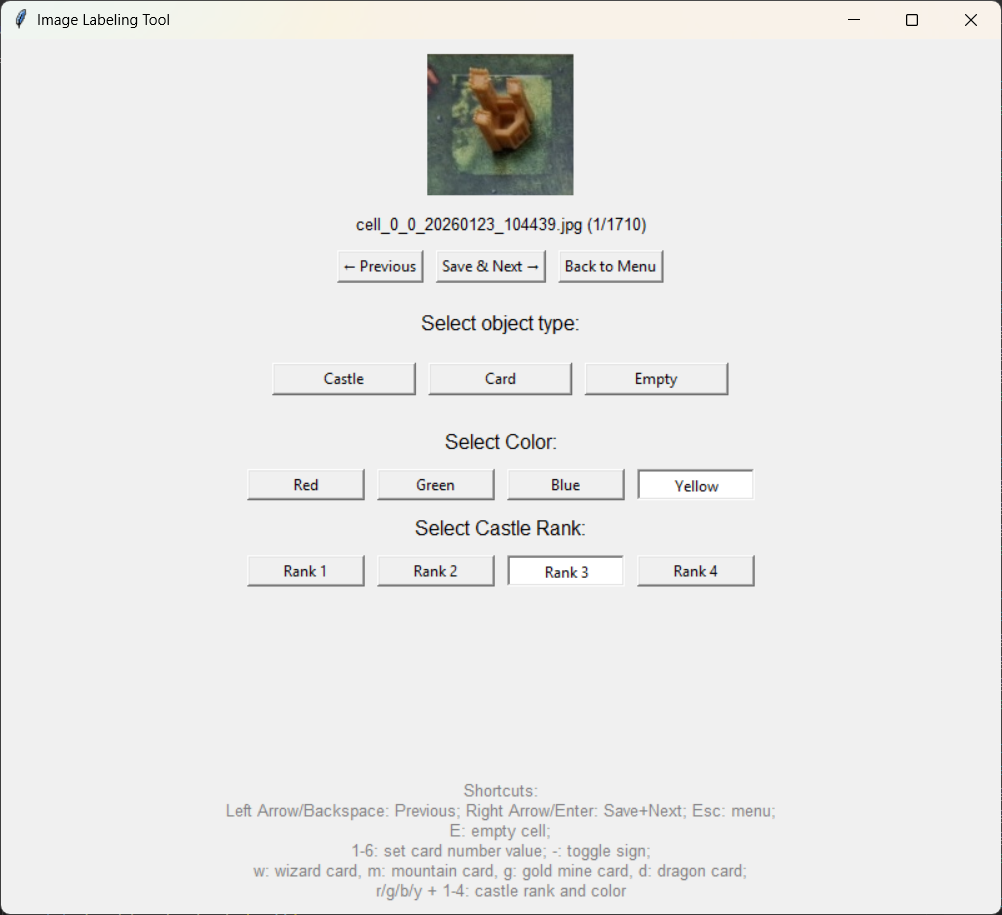
\includegraphics[width=1.0\linewidth]{figures/labeliranje_aplikacija.png} 
				\caption{Sučelje aplikacije za označavanje podataka.}
				\label{slk:oznacavanje}
			\end{figure}
		
		\subsection{Karakteristike konačnog skupa podataka}
		\label{podpog:karakteristike_podataka}
			Konačan skup podataka za učenje napravljen je od 57 originalnih slika igraće ploče. S obzirom na to da svaka ploča sadrži 30 polja, konačan skup se sastoji od 1710 slika pojedinačnih polja. Konkretnije, u skupu podataka za učenje postoji:
			\begin{itemize}
				\item 39 slika svake kartice s negativnim brojevnim vrijednostima (ukupno 234 slike),
				\item 42 slike svake kartice s pozitivnim brojevnim vrijednostima (ukupno 252 slike),
				\item 45 slika svake kartice s posebnim efektom (ukupno 180 slika),
				\item 48 slika dvoraca ranga 1 svake boje (ukupno 192 slike),
				\item 42 slike svakog dvorca ranga 2, 3 i 4 u svim bojama (ukupno 504 slike) te
				\item 348 slika praznih polja.
			\end{itemize}
			
			Ovaj skup podataka nije naročito velik prvenstveno zbog vremenskih ograničenja ovog rada. Ovo je pogotovo izraženo u konkretnim klasifikacijskim problemima u kojima se niti ne koristi cijeli skup podataka. Izrada većeg skupa podatak bi zahtijevala više vremena za pripremu i fotografiranje ploče te za označavanje. S obzirom na to skup podataka je ostao na ovoj veličini, ali postojeći radni okvir koji je razvijen u ovom radu omogućuje jednostavno proširivanje trenutačnog skupa.
		
		\subsection{Podjela podataka}
		\label{podpog:podjela_podataka}
			Cijeli skup podataka je podijeljen na tri dijela: 
			\begin{itemize}
				\item skup za treniranje koji čini 65\% cijelog skupa (1102 slika),
				\item skupa validaciju koji čini 20\% cijelog skupa (327 slika) te
				\item skup za testiranje koji čini preostalih 15\% skupa (281 slika).
			\end{itemize}
			
			Ovaj omjer podjele na skup za treniranje, validaciju i testiranje je očuvan kroz svaku klasu. To znači da je podjela u ovom omjeru zapravo napravljena na razini svake postojeće klase.
			
			Nakon podjele na skup za učenje, validaciju i testiranje iz svakog od ovih skupova su napravljeni pogledi koji će se zapravo koristiti u svakom od klasifikacijskih problema. Pogledi su samo filtrirani podaci s izdvojenim relevantnim oznakama za konkretan klasifikacijski problem. U nastavku su navedeni izrađeni pogledi za svaki od skupova.
			\begin{itemize}
				\item \textit{all} - sadrži sve slike, a izdvojena je oznaka tipa objekta (\textit{empty}, \textit{card} i \textit{castle}).
				\item \textit{cards} - sadrži slike kartica, a izdvojena je oznaka vrste kartice (\textit{number} i \textit{special}).
				\item \textit{castles\_color} - sadrži slike dvoraca, a izdvojena je oznaka boje dvorca (\textit{red}, \textit{green}, \textit{blue} i \textit{yellow}).
				\item \textit{castles\_rank} - sadrži slike dvoraca, a izdvojena je oznaka ranga dvorca (\textit{1}, \textit{2}, \textit{3} i \textit{4}).
				\item \textit{number\_cards} - sadrži slike kartica s brojevnim vrijednostima, a izdvojena je oznaka vrijednosti kartice (vrijednosti od \textit{-6} do \textit{-1} i od \textit{1} do \textit{6}).
				\item \textit{special\_cards} - sadrži slike posebnih kartica, a izdvojena je oznaka konkretne posebne kartice (\textit{dragon}, \textit{gold mine}, \textit{mountain} i \textit{wizard}).
			\end{itemize}
		
	\section{Augmentacija}
	\label{pog:augmentacija}
		Kako bi se djelomično kompenzirala mala veličina i potencijalno nedovoljna raznolikost napravljenog skupa podataka dodatno je korištena tehnika augmentacije podataka. Augmentacija podataka je metoda koja se u strojnom učenju manifestira kao generiranje modificiranih kopija već postojećih podataka~\cite{IBMDataAugmentation}. Cilj augmentacije je povećanje veličine i raznolikosti skupa podataka~\cite{IBMDataAugmentation}. Augmentacije koje su korištene u ovo radu su opisane u nastavku. Primjer originalne slike i primijenjenih pojedinačnih augmentacija koje su korištene u ovom radu prikazani su na slici~\ref{slk:augmentacije_zasebno} u pravilnoj rešetki od 3 reda i 4 stupca. Originalna slika se nalazi u prvom redu u prvom stupcu slike. Dodatno, primjer s primijenjenim nasumičnim kombinacijama augmentacija, kako su korištene prilikom treniranja modela, vidljiv je na slici~\ref{slk:augmentacije_nasumicno}. 
		
		\begin{figure}[htb]
			\centering
			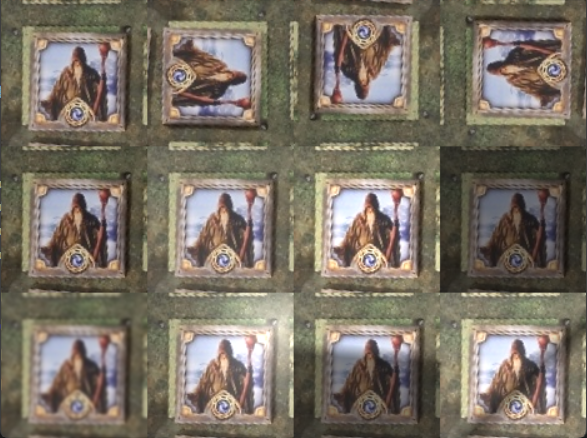
\includegraphics[width=0.6\linewidth]{figures/augmentacije_odvojeno.png} 
			\caption{Primjer pojedinačnih augmentacija.}
			\label{slk:augmentacije_zasebno}
		\end{figure}

		\begin{figure}[htb]
			\centering
			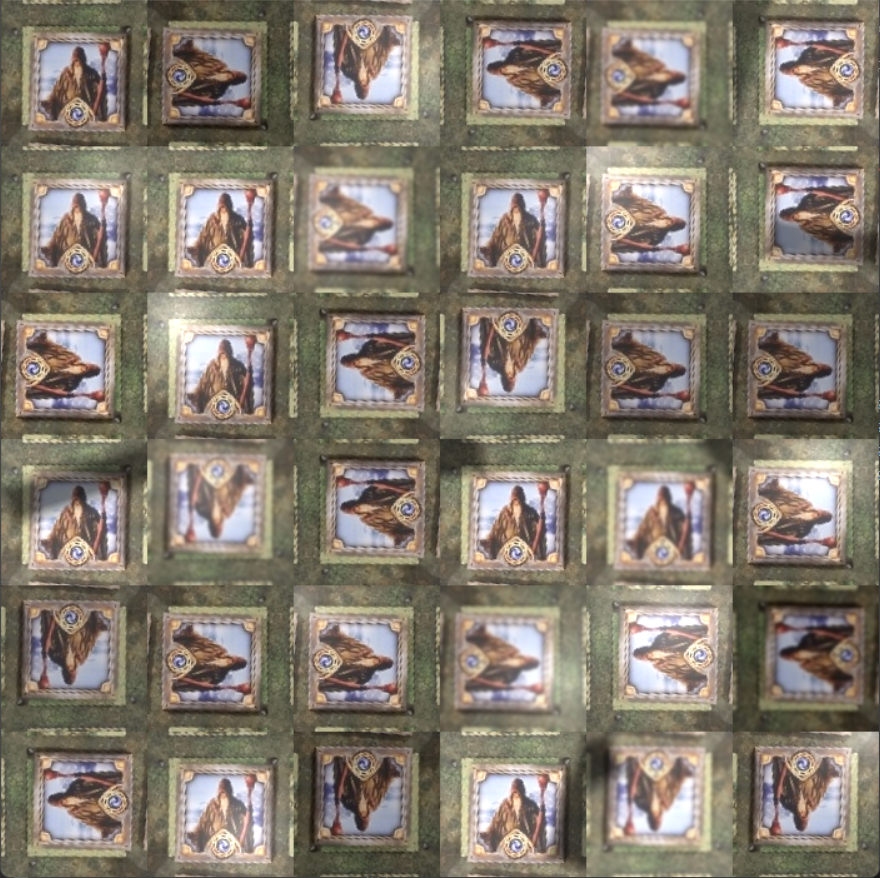
\includegraphics[width=1.0\linewidth]{figures/augmentacije_nasumicno.png} 
			\caption{Primjer nasumičnih kombinacija augmentacija.}
			\label{slk:augmentacije_nasumicno}
		\end{figure}
	
		\subsection{Rotacija}
			Rotacija je jedna od osnovnih i najjednostavnijih augmentacija koje su korištene u ovom radu. Konkretno su korištene rotacije za $90^\circ$, $180^\circ$ i $270^\circ$. Obrazloženje za korištenje rotacije je činjenica da igrači mogu elemente postavljati u različitim orijentacijama. Razlog za korištenje samo navedena tri kuta za rotaciju je prije svega što su slike pravokutne te bi se rotiranjem za neku drugu količinu stupnjeva dobila nepravilna slike koja bi vjerojatno narušila kvalitetu predikcije modela. Dodatno, kartice koje se postavljaju na ploču su obično postavljene u jednoj od tri navedene orijentacije uz blaga odstupanja, tako da je ovaj izbor bio logičan. Vjerojatnost korištenja rotacije prilikom augmentiranja slike je 75\% uz uniformnu vjerojatnost odabira jednog od tri moguća kuta rotacije. Primjeri rotirane originalne slike mogu se vidjeti na slici~\ref{slk:augmentacije_zasebno} u prvom redu.
		
		\subsection{Kontrast i svjetlina}
			Promjena kontrasta ostvaruje se skaliranjem vrijednosti svih piksela za zadani faktor. Faktor skaliranja se odabire prema uniformnoj distribuciji na intervalu $[0.8, 1.2]$. Na slici~\ref{slk:augmentacije_zasebno} prikazani su primjeri pojačavanja i smanjenja kontrasta. Primjer pojačanja kontrasta s faktorom skaliranja iz uniformne distribucije na intervalu $[1.1, 1.5]$ je vidljiv u drugom redu u trećem stupcu, dok je primjer smanjenja kontrasta s faktorom skaliranja iz uniformne distribucije na intervalu $[0.5, 0.9]$ vidljiv u drugom redu u četvrtom stupcu.
		
			Promjena svjetline se ostvaruje dodavanjem zadane vrijednosti na vrijednost svakog piksela. Vrijednost koja se dodaje na svaki piksel odabire se relativno s obzirom na prosječnu svjetlinu piksela slike. Ta vrijednost se računa tako da se odabere faktor iz uniformne distribucije kojim se množi svjetlina slike. Svjetlina slike je izračunata kao prosječna vrijednost svih piksela u slici po svim kanalima. Primjeri smanjivanja i pojačavanja svjetline su vidljivi na slici~\ref{slk:augmentacije_zasebno} u drugom redu u prvom i drugom stupcu. Za smanjivanje svjetline na primjeru se koristio faktor iz uniformne distribucije na intervalu $[0.6, 1.0]$, dok se za pojačavanje svjetline na primjeru koristio faktor iz uniformne distribucije na intervalu $[1.0, 1.4]$.
			
			Interval uniformne distribucije je početno postavljen na $[0.8, 1.2]$. Ako je pak svjetlina slike iznad unaprijed određenog gornjeg praga svjetline, uzima se interval $[0.65, 1.05]$. Cilj je spriječiti stvaranje slike koja je neprirodno presvijetla. Ako je pak svjetlina slike ispod unaprijed određenog donjeg praga svjetline, uzima se interval $[0.95, 1.35]$. Cilj je spriječiti pretjerano tamne slike koje djeluju neprirodno.
			
			Prilikom augmentiranja slike promjena kontrasta i svjetline se direktno primjenjuje s vjerojatnošću od 40\% ako se ne provodi dodavanje odsjaja. Augmentacija promjene svjetline i kontrasta se također ponekad koristi u sastavu dodavanja odsjaja i sjene kako bi se karakteristike slike prilagodile tim augmentacijama.
		
		\subsection{Zamućenje}
			Zamućenje se ovdje ostvaruje primjenom Gaussovog filtra s veličinom jezgre $5x5$. Vjerojatnost primjene zamućenja prilikom augmentiranja slike iznosi 25\%. Primjer primijenjenog zamućenja može se vidjeti na slici~\ref{slk:augmentacije_zasebno} u trećem redu u prvom stupcu.
		
		\subsection{Odsjaj}
			Odsjaj je simuliran kao točkasto područje koncentrirano visokog osvjetljenja koje se kružno raspršuje okolo. Kod odsjaja se koriste parametri navedeni u nastavku.
			\begin{itemize}
				\item Intenzitet ($i$) - jačina odsjaja; odabire se iz uniformne distribucije na intervalu $[0.2, 0.55]$.
				\item Centar odsjaja ($x_c, y_c$) - relativna pozicija s obzirom an dimenzije slike; odabire se iz uniformne distribucije nad $[0.0, 1.0]^2$.
				\item Raspršenje ($s$) - određuje koliko se odsjaj širi, to jest koliko intenzitet odsjaja brzo opada; odabire se iz uniformne distribucije na intervalu $[2, 4]$.
			\end{itemize}
			
			Nakon slučajnog odabira parametara računa se trenutačna svjetlina slike kako je opisano ranije. Ako je svjetlina iznad gornjeg praga svjetline vrijednost intenziteta se prepolavlja kako bi se spriječilo stvaranje presvijetle slike. Ako je pak svjetlina ispod donjeg praga svjetline radi se nasumična promjena kontrasta i svjetline. Interval uniformne distribucije za promjenu svjetline je $[srednji\_prag / svjetlina, srednji\_prag / svjetlina + 0.15]$, gdje je $srednji\_prag$ srednja vrijednost gornjeg i donjeg praga svjetline. Interval za kontrast je pak $[1.05, 1.2]$.
			
			Nakon ovih modifikacija računaju se točne koordinate centra odsjaja te se za svaku poziciju na slici računa udaljenost od centra odsjaja. Definira se maksimalna teoretska udaljenost kao $d_{max} = \sqrt{visina^2 + sirina^2}$. Računa se maska za svaku poziciju piksela prema formuli $maska = (1 - d / d_{max})^s$, gdje je $d$ udaljenost piksela od centra odsjaja, $d_{max}$ prije definirana maksimalna teoretska udaljenost te $s$ raspršenje. Vrijednosti u maski se zatim množe s uzorkovanim intenzitetom te maksimalnom vrijednosti piksela (255). Završno se nova slika računa dodavanjem maske na originalnu sliku.
			
			Vjerojatnost dodavanja odsjaja na sliku tijekom provođenja augmentacije je 40\%. Primjer dodanog odsjaja vidljiv je na slici~\ref{slk:augmentacije_zasebno} u trećem redu u drugom stupcu.
		
		\subsection{Sjene}
			Sjene se na slikama polja mogu pojaviti prilikom jakog osvjetljenja zbog prisutnosti raznih objekata u okolini. Najizraženije sjene koje se mogu pojaviti u ovom kontekstu su sjene koje bacaju dvorci postavljeni na ploču te veliki objekti u okolini ploče, kao na primjer drugi igrači. Pretpostavka je da će u prvom slučaju sjena na slici obično ličiti na relativno debelu liniju, dok će se u drugom obično manifestirati tako da cijelo područje s otprilike jedne strane pravca bude u sjeni. U nastavku rada se na prvi tip sjene referira kao linijska sjena, a drugi tip kao poluprostorna sjena. Ovo su naravno jako grube aproksimacije ali ovakve pretpostavke jako olakšavaju modeliranje sjena.
			
			Prilikom generiranja sjena prvo se provjerava svjetlina slike koja se augmentira. Ako je svjetlina iznad gornjeg praga, dodavanje sjene se preskače. Opravdanje za ovaj pristup je sljedeći - ako je slika već dovoljno svjetla, vjerojatno se radi o okruženju s jakim osvjetljenjem, a prilikom jakog osvjetljenja obično su već prisutne izražene sjene. Zbog toga bi kod takvih slika s postojećim sjenama dodavanje umjetnih sjena moglo izgledati dosta neprirodno. Ako je svjetlina ispod donjeg praga, na sliku se primjenjuje promjena kontrasta i svjetlina na identičan način kao i kod dodavanja odsjaja.
			
			Dva parametra koja opisuju obje vrste sjena su intenzitet i oštrina. Intenzitet opisuje koliko je sjena tamna te se slučajno odabire iz uniformne distribucije na $[0.4, 0.65]$. Oštrina opisuje relativnu oštrinu prijelaza iz područja izvan sjene u područja u sjeni u odnosu na dimenzije slike te se slučajno odabire iz uniformne distribucije na $[0.06, 0.09]$. Linijska sjena ima dodatan parametar relativne širine linije sjene u odnosu na dimenzije slike te se ona slučajno odabire iz uniformne distribucije na $[0.15, 0.4]$. Nakon odabira relativne oštrine i relativne širine ti parametri se množe s duljinom dijagonale slike kako bi se dobile vrijednosti pravih parametara.
			
			Nakon odabira parametara radi se prilagodba kontrasta i svjetline slike. Kontrast se povećava za faktor $1+intenzitet/4$, dok se svjetlina povećava za slučajan broj iz intervala $[10, \lfloor svjetlina*intenzitet/2 \rfloor]$.
			
			Za poluprostorne sjene idući je korak odabir dviju slučajnih točaka koje će definirati pravac koji će biti granica sjene. Zatim se računa mapa apsolutne udaljenosti svih piksela od definiranog pravca. Vrijednosti u mapi udaljenosti se zatim ograničavaju odozgo s vrijednošću apsolutne oštrine. Ovime se kontrolira koliko će biti širok pojas prijelaza iz osvijetljenog područja do područja potpune sjene. Nakon toga se vrijednosti u mapi dijele s vrijednošću apsolutne oštrine kako bi se vrijednosti skalirale na interval $[0, 1]$. Ovako dobivena mapa se zatim množi s intenzitetom sjene. Konačna slika se dobiva množenjem originalne slike s vrijednostima u komplementarnoj maski koja se dobiva kao $1-maska$. Rezultat primjene ovakve augmentacije je vidljiv na slici~\ref{slk:augmentacije_zasebno} u trećem redu u trećem stupcu.
			
			Kod linijskih sjena idući je korak odabir nasumične točke na slici te nasumičnog kuta. Odabrana točka će biti jedna krajnja točka linije, dok će odabrani kut definirati suprotan smjer od smjera u kojem će linija biti orijentirana od odabrane točke prema rubu slike. Iz odabrane točke i kuta računaju se parametri pripadnog pravca te okomitog pravca koji prolazi kroz odabranu točku. Za originalni pravac računa se maska apsolutne udaljenosti od pravca dok se za okomiti pravac računa maska predznačne udaljenosti. Ove dvije maske se zatim kombiniraju tako da se na svakoj poziciji odabire veća vrijednost iz danih maski. Novodobivena maska se zatim modificira tako da se vrijednost svake pozicije oduzme od polovice vrijednosti odabrane širine linije. Konačna maska se dobiva ograničavanjem vrijednosti maske na interval $[0, ostrina]$ kako bi se kontrolirala širina prijelaza sjene. Zatim se vrijednosti maske dijele s oštrinom kako bi se vrijednosti ograničile na interval $[0, 1]$. Konačna slika se ponovno dobiva množenjem originalne slike s vrijednostima u komplementarnoj maski koja se dobiva kao $1-maska$. Primjer ovakve augmentacije je vidljiv na slici~\ref{slk:augmentacije_zasebno} u trećem redu u četvrtom stupcu.
			
			Vjerojatnost dodavanja sjene na sliku tijekom provođenja augmentacije je 60\% ako se ne provodi dodavanje odsjaja niti direktna promjena kontrasta i svjetline. Od toga se linijska sjena pojavljuje u 50\% slučajeva, dok se u ostalih 50\% slučajeva pojavljuje poluprostorna sjena.

	\section{Klasifikacijski modeli}
	\label{pog:klasifikacija}
		
		Kao što je prije rečeno, za klasifikaciju objekata na pojedinim poljima koriste se metode dubokog učenja. Vjerojatno najjednostavniji pristup bio bi uzeti postojeći predtrenirani model te ga prilagoditi i dotrenirati za klasifikaciju objekata na poljima ove igre. Međutim, mana takvog pristupa je da se koriste modeli koji su pretjerano veliki, a samim time i sporiji te zahtjevniji za treniranje. Naprimjer, najmanji dostupan \textit{ResNet} model u programskoj biblioteci \textit{PyTorch}, \textit{ResNet18} ima veličinu od 44.7 MB~\cite{ResNet18} te skoro 11.7 milijuna parametara~\cite{ResNet18}. Iako bi korištenje i lokalno dotreniranje takvog modela bilo izvedivo, drugim pristupom moguće je ostvariti željene rezultate s ukupno manjim brojem parametara i značajno manjim modelima.
		
		Ideja koja se koristi u ovom radu je rastav problema klasifikacije na više koraka. U svakom koraku se rješavaju klasifikacijski potproblemi koji zajedno rješavaju početni problem. U tu svrhu potrebno je koristiti više klasifikacijskih modela - po jedan za svaki potproblem. Rezultat ovakvog pristupa su mali i kompaktni modeli koji ne zahtijevaju puno resursa za treniranje, ali imaju vrlo visoke performanse u kontekstu točnosti predikcija. Konkretno, rezultantni \textit{PyTorch} modeli imaju ukupnu veličinu od oko 4 MB te oko 500000 parametara. Ovo je bitno jer je cilj ovog rada razviti aplikaciju koja će raditi potpuno lokalno bez spajanja na vanjske servise. Zbog toga je bitno da korišteni modeli budu mali i brzi kako bi aplikacija bila što efikasnija na mobilnim uređajima.
		
		Konkretan proces klasifikacije koristi 6 dubokih modela. Prvi model donosi odluku o vrsti objekta na konkretnom polju. Model odlučuje između kartice, dvorca i praznog polja. Ako je prvi model klasificirao objekt kao prazno polje, onda je to konačan rezultat. Ako je objekt klasificiran kao dvorac, slijedi predikcija dva modela - jedan klasificira dvorac prema boji, a drugi prema njegovom rangu. Ako je objekt klasificiran kao kartica, slijedi odluka modela koji klasificira kartice u posebne kartice i kartice s brojevima (numeričke kartice). Ako je taj model klasificirao karticu kao numeričku, slijedi odluka modela koji klasificira numeričke kartice na temelju njihovih brojeva. U suprotnom slijedi model koji klasificira posebne kartice. Ovi modeli koriste pripadne prilagođene poglede definirane u potpoglavlju \ref{podpog:podjela_podataka}.
		
		\subsection{Arhitekture modela}
		\label{podpog:arhitektura_modela}
			Svi korišteni modeli su dizajnirani prema istom arhitekturalnom obrascu. Prvi dio svakog modela čini modul za izlučivanje značajki koji se temelji na operacijama konvolucije. Nakon njega slijedi globalno sažimanje prosjekom kako bi model bio adaptivan s obzirom na dimenzije slike. Zadnji dio modela je linearna klasifikacijska glava.
			
			Svaki modul za izlučivanje značajki sastoji se od proizvoljnog broja složenih konvolucijskih blokova. Svaki konvolucijski blok sastoji se od 2-D konvolucije koja čuva prostorne dimenzije, sloja normalizacije nad grupom (\textit{engl. BatchNorm}), ReLU aktivacijske funkcije te opcionalnog 2x2 sloja sažimanja maksimumom. Broj izlaznih kanala svake konvolucije i veličina konvolucijske jezgre su podesiv kod instanciranja pojedinog bloka. Na slici~\ref{podslk:konv_blok} je vidljiv shematski dijagram konvolucijskog bloka.
			
			Svaka klasifikacijska glava sastoji se od proizvoljnog broja linearnih slojeva. Nakon svakog linearnog sloja, osim zadnjeg, slijede ReLU aktivacijska funkcija te opcionalni sloj za nasumično isključivanje neurona (\textit{engl. Dropout layer}). Sloj za nasumično isključivanje je regularizacijska tehnika u kojoj se nasumični neuroni isključuju tijekom treniranja~\cite{GeeksForGeeksDropout}. Cilj ove tehnike je smanjiti međuzavisnosti između neurona i time poboljšati generalizaciju~\cite{GeeksForGeeksDropout}. Izvan faze treniranja ovaj sloj nema utjecaj na rad modela~\cite{GeeksForGeeksDropout}. Dimenzije pojedinog linearnog sloja i stopa isključivanja se definiraju tijekom instanciranja sloja. Na slici~\ref{podslk:lin_blok} je prikazan shematski dijagram opisanog linearnog bloka.
			
			\begin{figure}[htbp]
				\centering
				
				\begin{subfigure}{0.45\textwidth}
					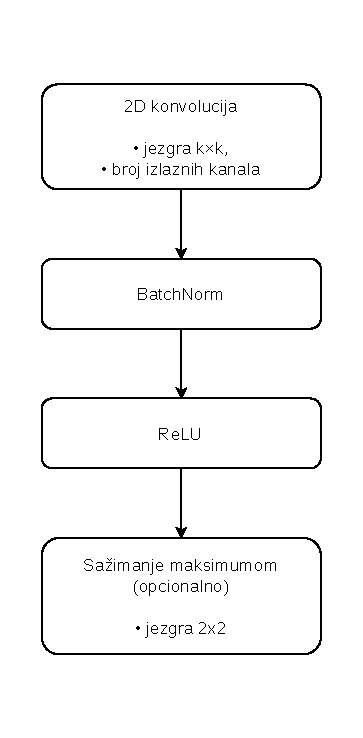
\includegraphics[width=\linewidth]{figures/konv_blok2.drawio.pdf}
					\caption{Dijagram konvolucijskog bloka.}
					\label{podslk:konv_blok}
				\end{subfigure}
				% \hfill
				\begin{subfigure}{0.45\textwidth}
					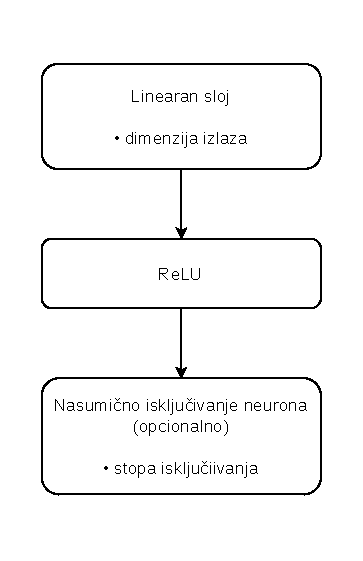
\includegraphics[width=\linewidth]{figures/lin_blok1.drawio.pdf}
					\caption{Dijagram linearnog bloka.}
					\label{podslk:lin_blok}
				\end{subfigure}
				
				\caption{Shematski dijagrami gradivnih blokova klasifikacijskih modela.}
				\label{slk:gradivni_blokovi}
			\end{figure}
			
			Konkretne arhitekture pojedinih modela prikazane su u tablici \ref{tab:cnn_arhitekture}.
		
			\begin{table}[htb]
				\centering
				\caption{Pregled arhitektura konvolucijskih modela.}
				\label{tab:cnn_arhitekture}
				
				\begin{adjustbox}{width=0.94\textwidth}
					\begin{tabular}{cccccc}
						\toprule
						\makecell{\textbf{Model}} &
						\makecell{\textbf{Broj}\\\textbf{izlaznih}\\\textbf{kanala}\\\textbf{konvolucija}} &
						\makecell{\textbf{Veličina}\\\textbf{konvolucijskih}\\\textbf{jezgri}} &
						\makecell{\textbf{Prisutnost}\\\textbf{sloja}\\\textbf{sažimanja}} &
						\makecell{\textbf{Dimenzije}\\\textbf{linearnih}\\\textbf{slojeva}} &
						\makecell{\textbf{Broj}\\\textbf{parametara}} \\ 
						\midrule
						
						\makecell{Model za\\razlikovanje\\kartica, dvoraca i\\praznih polja}
						& 12, 24, 36 & 3x3, 3x3, 3x3 & +, +, + & 48 & 12831 \\[9mm]
						
						\makecell{Model za\\klasifikaciju\\boje dvorca}
						& 24, 24 & 3x3, 3x3 & +, + & 48 & 7372 \\[9mm]
						
						\makecell{Model za\\klasifikaciju\\razine dvorca}
						& \makecell{80, 80,\\72, 72,\\72, 72, 72} & \makecell{7x7, 5x5,\\3x3, 3x3,\\3x3, 3x3, 3x3} & \makecell{-, +,\\-, +,\\-, +, -} & 64 & 416716 \\[9mm]
						
						\makecell{Model za\\razlikovanje\\posebnih kartica i\\kartica s brojevima}
						& 24, 24, 36 & 3x3, 3x3, 3x3 & +, +, + & 48 & 38760 \\[9mm]
						
						\makecell{Model za\\klasifikaciju\\posebnih kartica}
						& 32, 24 & 3x3, 3x3 & +, + & 48 & 15734 \\[9mm]
						
						\makecell{Model za\\klasifikaciju\\kartica s brojevima}
						& \makecell{36, 36,\\36, 36} & \makecell{3x3, 3x3,\\3x3, 3x3} & \makecell{+, +,\\+, +} & 48 & 9340 \\
						
						\bottomrule
					\end{tabular}
				\end{adjustbox}
			\end{table}
			
		\subsection{Treniranje modela}
			Tijekom učenja koristi se gubitak unakrsne entropije, dok se za optimizaciju koristi Adam optimizator. Adam je optimizacijska tehnika koja kombinira moment gradijenta i adaptivnu stopu učenja za svaki parametar~\cite{GeeksForGeeksAdam}. Ovime se postiže stabilnije učenje i često jednostavnije podešavanje hiperparametara u odnosu na stohastički gradijentni spust~\cite{GeeksForGeeksAdam}. Uz Adam optimizator koristi se i L2 regularizacija koja se manifestira u hiperparametru iščezavanja težina (\textit{engl. weight decay}). Konkretne konfiguracije za treniranje pojedinog modela su vidljive u tablici \ref{tab:cnn_hiperparametri}.
			
			\begin{table}[htb]
				\centering
				\caption{Pregled hiperparametara korištenih pri treniranju klasifikacijskih modela.}
				\label{tab:cnn_hiperparametri}
				
				\begin{adjustbox}{width=0.94\textwidth}
					\begin{tabular}{ccccccc}
						\toprule
						\makecell{\textbf{Model}} &
						\makecell{\textbf{Veličina}\\\textbf{grupe}} &
						\makecell{\textbf{Stopa}\\\textbf{učenja}} &
						\makecell{\textbf{Koeficijent}\\\textbf{regularizacije}} &
						\makecell{\textbf{Broj}\\\textbf{epoha}} &
						\makecell{\textbf{Broj}\\\textbf{augmentacija}\\\textbf{po slici}} &
						\makecell{\textbf{Stopa}\\\textbf{gašenja}\\\textbf{neurona}} \\ 
						\midrule
						
						\makecell{Model za razlikovanje\\kartica, dvoraca i\\praznih polja}
						& 32 & 0.0001 & 0.00005 & 100 & 27 & 0.1 \\[7mm]
						
						\makecell{Model za klasifikaciju\\boje dvorca}
						& 32 & 0.0004 & 0.00005 & 50 & 20 & 0.2 \\[7mm]
						
						\makecell{Model za klasifikaciju\\razine dvorca}
						& 32 & 0.0001 & 0.0001 & 75 & 40 & 0.4 \\[7mm]
						
						\makecell{Model za razlikovanje\\posebnih kartica i\\kartica s brojevima}
						& 32 & 0.0005 & 0.0001 & 20 & 18 & 0.1 \\[7mm]
						
						\makecell{Model za klasifikaciju\\posebnih kartica}
						& 32 & 0.0002 & 0.0001 & 60 & 36 & 0.2 \\[7mm]
						
						\makecell{Model za klasifikaciju\\kartica s brojevima}
						& 32 & 0.0002 & 0.0000 & 60 & 25 & 0.1 \\
						
			            \bottomrule
					\end{tabular}
				\end{adjustbox}
			\end{table}
			
		\subsection{Odabir hipoteza i vrednovanje modela}
		\label{podpog:odabir_i_vrednovanje}
			% odabir modela ili hipoteze?
			Odabir konkretne hipoteze u procesu učenja se radi pomoću skupa za validaciju. Tijekom treniranja model se evaluira na validacijskom skupu nakon svake epohe učenja. Za evaluaciju se računa gubitak i točnost (\textit{engl. accuracy}). Nakon provedenog treniranja odabire se hipoteza koja je imala najbolju točnost na validacijskom skupu, a u slučaju više takvih hipoteza odabire se hipoteza s manjim gubitkom na validacijskom skupu.
			
			Za konačno vrednovanje modela koristi se skup za testiranje. Na skupu za testiranje se za odabranu hipotezu računa matrica konfuzije. Iz nje se zatim za svaku klasu računaju točnost, preciznost (\textit{engl. precision}), odziv (\textit{engl. recall}) te F1-mjera. Dodatno se računaju i mikro-uprosječenja navedenih mjera po klasama, s obzirom na to da je klasifikacija svakog primjera bila jednako važna neovisno o njegovoj klasi~\cite{Snajder2022VrednovanjeModela}.
			
			\begin{table}[htb]
				\centering
				\caption{Izmjerene mjere vrednovanja za odabrane modele na testnom skupu.}
				\label{tab:rezultati_modela}
				\begin{adjustbox}{width=0.84\textwidth}
					\begin{tabular}{ccccc}
						\toprule
						\textbf{Model} & \textbf{Točnost} & \textbf{Preciznost} & \textbf{Odziv} & \textbf{F1-mjera} \\
						\midrule
						
						\makecell{Model za razlikovanje kartica,\\ dvoraca i praznih polja} & 1.0000 & 1.0000 & 1.0000 & 1.0000 \\[5mm]
						\makecell{Model za klasifikaciju\\boje dvorca} & 1.0000 & 1.0000 & 1.0000 & 1.0000 \\[5mm]
						\makecell{Model za klasifikaciju\\razine dvorca} & 0.9914 & 0.9914 & 0.9914 & 0.9914 \\[5mm]
						\makecell{Model za razlikovanje posebnih\\kartica i kartica s brojevima} & 1.0000 & 1.0000 & 1.0000 & 1.0000 \\[5mm]
						\makecell{Model za klasifikaciju\\posebnih kartica} & 1.0000 & 1.0000 & 1.0000 & 1.0000 \\[5mm] % 0.9643 1.0000
						\makecell{Model za klasifikaciju\\kartica s brojevima} & 1.0000 & 1.0000 & 1.0000 & 1.0000 \\
						
						\bottomrule
					\end{tabular}
				\end{adjustbox}
			\end{table}
			
			Mikro-uprosječenja navedenih mjera vrednovanja na testnom skupu za svaki od odabranih modela vidljive su u tablici~\ref{tab:rezultati_modela}. Vrijedi opaziti da za svaki model sve mjere vrednovanja imaju istu vrijednost, što je posljedica korištenja mikro-uprosječenja mjera~\cite{Snajder2022VrednovanjeModela}. U tablici~\ref{tab:rezultati_modela} je vidljivo da su gotovo svi modeli ostvarili savršenu točnost. Jedina iznimka je model za klasifikaciju ranga dvorca. Tijekom treniranja se pokazalo da je to bio daleko najsloženiji klasifikacijski problem. To se odrazilo i u tome da je za taj problem korišten daleko najsloženiji model te je on pronađen kroz daleko najveći broj pokušaja - čak 40. Iako su ostali modeli ostvarili savršenu točnost na testnom skupu, taj rezultat treba uzeti sa zrnom soli. Naime, skup podataka za učenje koji se koristio kod treniranja je bio relativno mali. Stoga je vrlo moguće da su za neke modele ove procjene neprecizne. No unatoč tome s visokom razinom sigurnosti može se tvrditi da su prave točnosti naučenih modela vrlo visoke. Stoga su ovi rezultati u svakom slučaju zadovoljavajući.
			
			 % je kod svakog modela ostvarena vrlo visoka točnost na testnom skupu. Najlošiju ostvarenu točnost ima model za klasifikaciju posebnih kartica, ali treba napomenuti da je model zapravo napravio krivu klasifikaciju na samo jednom primjeru u testnom skupu. Tako veliki pad u točnosti radi samo jednog primjera je posljedica vrlo malog skupa za testiranje. Drugi model koji nije ostvario savršenu točnost jest model za klasifikaciju razine dvorca.  To je bilo posebno izraženo na nekim problemima, kao što je već rečeno na primjeru modela za klasifikaciju posebnih kartica.
			
	\section{Mobilna aplikacija za Android}
		Cijeli sustav je na kraju enkapsuliran u Android mobilnu aplikaciju. Mobilna aplikacija je zamišljena tako da može funkcionirati potpuno lokalno bez spajanja na vanjske servise. Varijanta s vanjskim servisom na poslužitelju u ovom kontekstu nema previše smisla zbog nepotrebnih komplikacija koje uvodi. Prije svega, takva varijanta bi zahtijevala pristup poslužitelju kojeg bi bilo potrebno konfigurirati. Iako danas postoje besplatne usluge javnih poslužitelja, kao na primjer \textit{Render}~\cite{Render}, one često pružaju ograničene performanse te se ne preporučuju za produkcijske aplikacije~\cite{Render}. U slučaju ozbiljnog korištenja aplikacije ovakav pristup bi vjerojatno značajno srozao performanse cijelog sustava. Također, ovakva varijanta bi zahtijevala internetsku vezu prema centralnom poslužitelju, što je nepotrebna ovisnost. Dodatno, kompletna logika i duboki modeli cijele aplikacije su dovoljno jednostavni te ne predstavljaju pretjerano memorijsko i procesorsko opterećenje za mobilne uređaje. Zbog svega navedenog, razvoj mobilne aplikacije s odvojenim vanjskim servisom ne donosi nikakve praktične prednosti, a uvodi nepotrebne slabosti u cijeli sustav. Zbog toga je i takva ideja razvoja odbačena.
		
		Aplikacija je napravljena na način da korisniku nudi dva režima rada za praćenja igre. Jedan način omogućuje korisniku praćenje rezultata cijele igre kroz sve tri runde. Ovaj režim omogućuje korisniku da koristi aplikaciju za cjelokupno praćenje igre i maksimalno iskoristi mogućnosti aplikacije. Drugi način omogućuje korisniku jednokratan pregled stanja ploče neovisno o trenutačnoj fazi igre. Ovaj režim omogućuje da korisnik koristi aplikaciju kao pomoćni alat. Dodatno, ovim načinom rada korisnik može provjeravati stanje ploče usred runde, što mu može pomoći u donošenju odluka tijekom igre. Na slici~\ref{slk:zasloni_aplikacije}a vidljiv je početni zaslon aplikacije na kojem se bira jedan od dva režima rada.
		
		U prvom načinu rada korisnik na kraju svake runde fotografira ploču ili učitava već postojeću fotografiju iz galerije mobitela. Na slici~\ref{slk:zasloni_aplikacije}b se vidi zaslon na kojem korisnik bira na koji način će piložiti sliku. Aplikacija koristi sustav za detekciju ploče opisan u poglavlju~\ref{pog:detekcija}. Detektirana ploča se prikazuje na zaslonu kao na slici~\ref{slk:zasloni_aplikacije}c. S obzirom na to da sustav može griješiti, korisnik mora potvrditi detektiranu ploču ili ponovno priložiti fotografiju fotografiranjem ili učitavanjem fotografije. Nakon što korisnik potvrdi detektiranu ploču aplikacija koristi modele iz tablice~\ref{tab:cnn_arhitekture} na način opisan u poglavlju~\ref{pog:klasifikacija}. Dobivene predikcije se koriste se za izradu modela ploče koji se prikazuje korisniku, kao na slici~\ref{slk:zasloni_aplikacije}d. Korisnik može pregledati prikazane predikcije. S obzirom na to da klasifikacijski modeli mogu pogriješiti, korisniku je omogućeno i uređivati predložene predikcije. Korisnik nakon opcionalnog uređivanja može potvrditi predikcije. Nakon potvrde aplikacija primjenjuje pravila igre kako bi izračunala bodove svakog igrača. Izračunati bodovi se prikazuju korisniku zajedno sa prijašnjim bodovima te ukupnom sumom za svakog igrača, kao što je vidljivo na slici~\ref{slk:zasloni_aplikacije}e. Ovaj krug se ponavlja tri puta, jednom za svaku rundu. Na kraju treće runde i prikaza bodova aplikacija proglašava pobjednika, nakon čega se vraća na početni zaslon.
		
		\begin{figure}[htbp]
			\centering
			
			\begin{subfigure}{0.30\textwidth}
				
\includegraphics[width=\linewidth]{figures/app_main.jpg}
				\caption{Početni zaslon Android aplikacije.}
				\label{podslk:applikacija_glavni}
			\end{subfigure}
			\hspace{1.2em}
			\begin{subfigure}{0.30\textwidth}
				
\includegraphics[width=\linewidth]{figures/photo_menu.jpg}
				\caption{Zaslon izbora načina pružanja fotografije.}
				\label{podslk:izbor_slike}
			\end{subfigure}
			\hspace{1.2em}
			\begin{subfigure}{0.30\textwidth}
				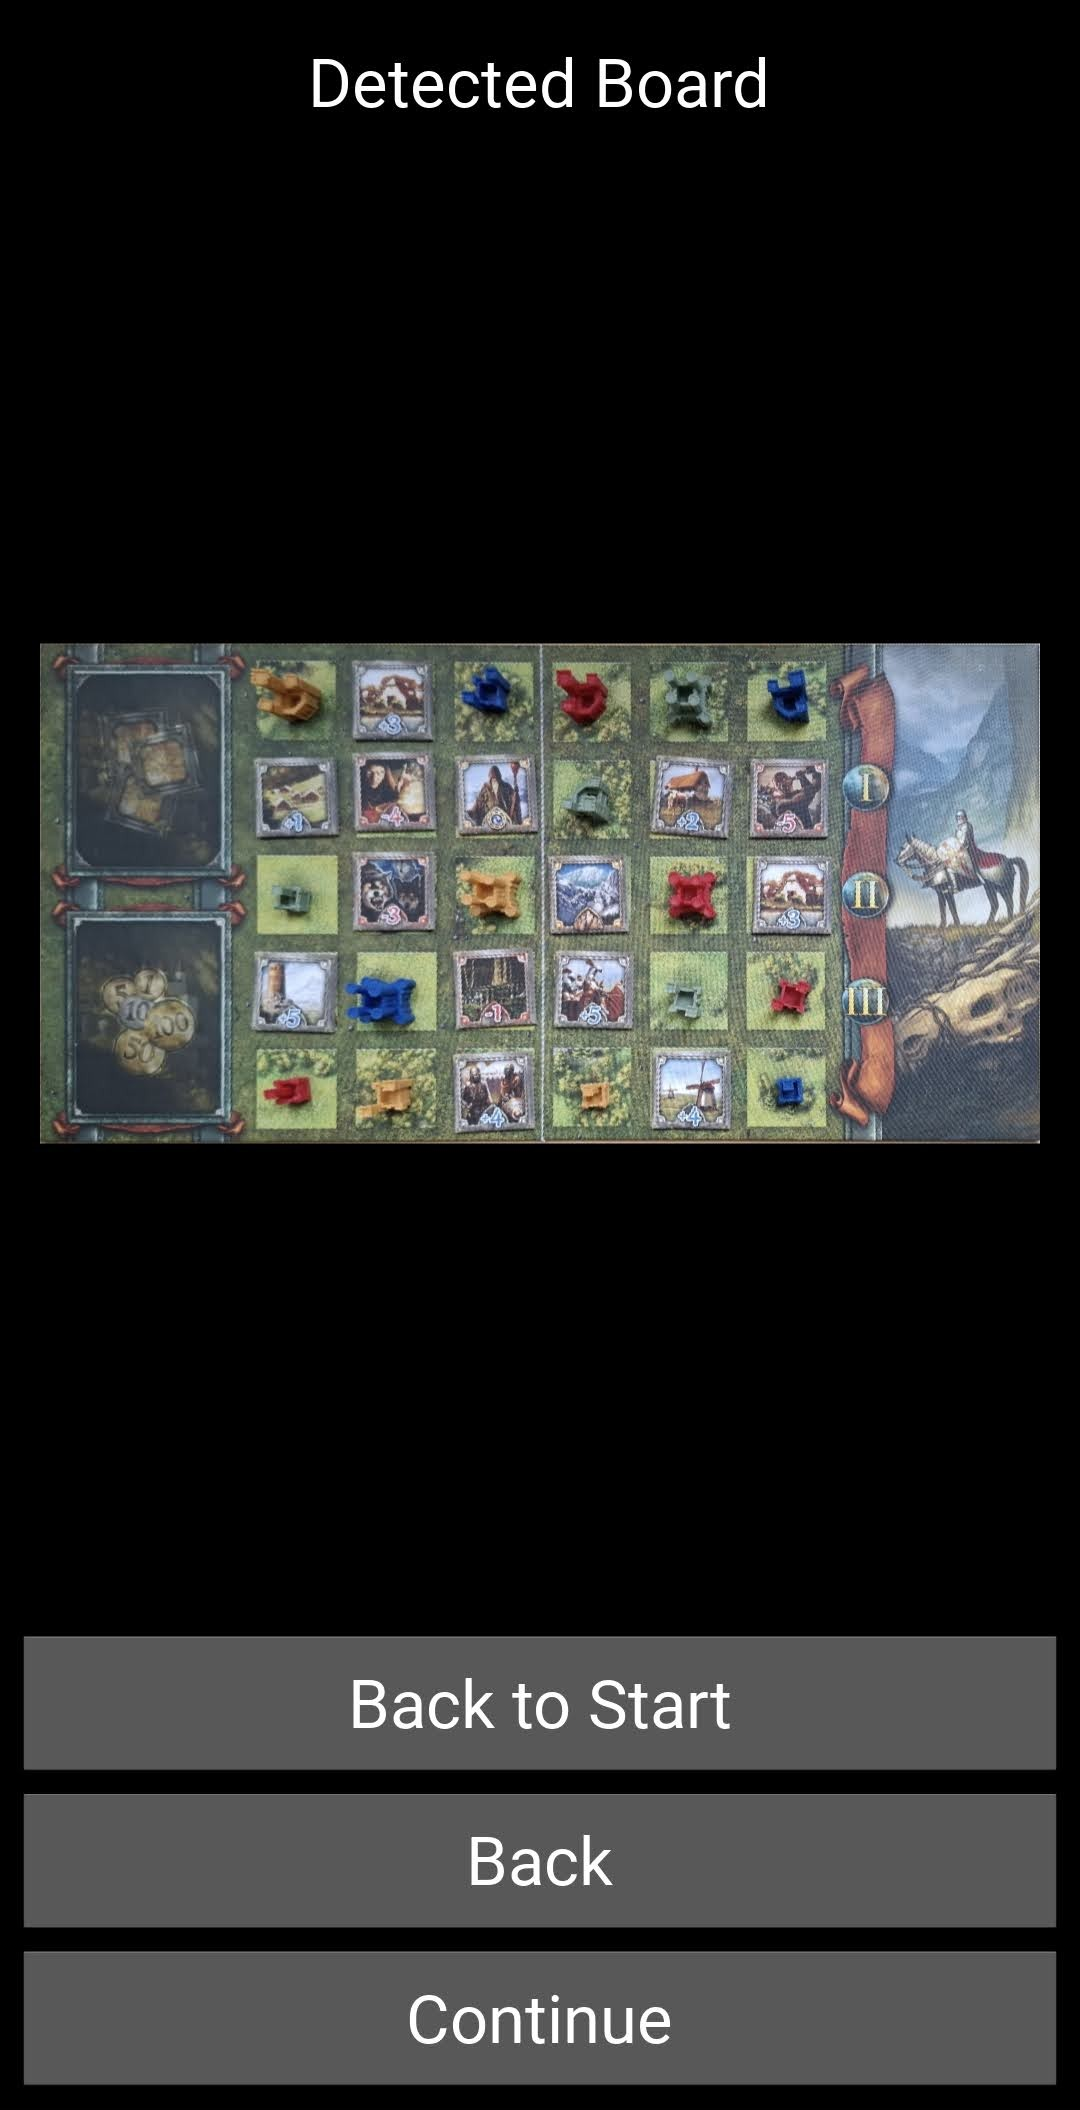
\includegraphics[width=\linewidth]{figures/detected_board.jpg}
				\caption{Zaslon s prikazom detektirane ploče.}
				\label{podslk:detektirana_ploca}
			\end{subfigure}
			
			\vspace{0.6em}
			
			\begin{subfigure}{0.30\textwidth}
				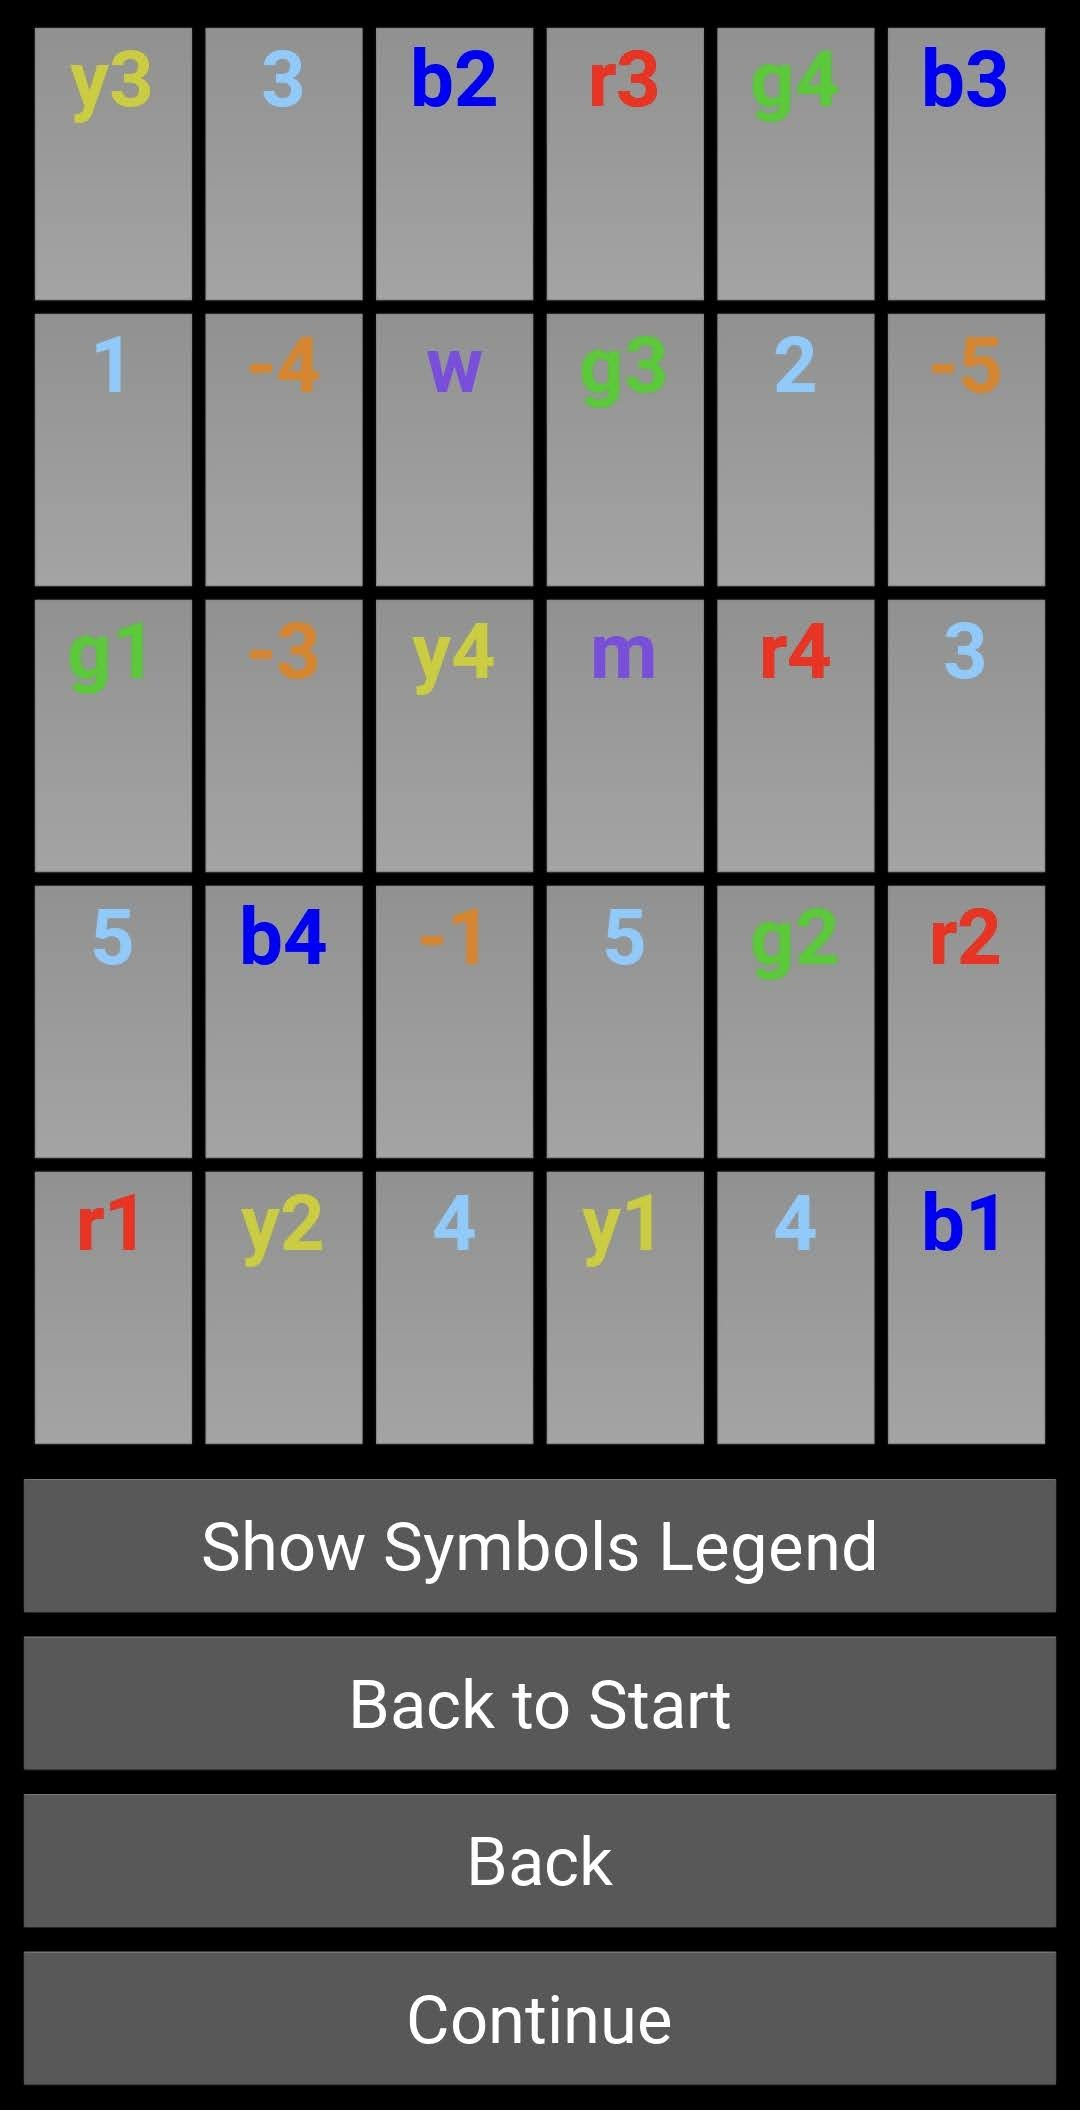
\includegraphics[width=\linewidth]{figures/board_model.jpg}
				\caption{Zaslon s prikazom modela ploče.}
				\label{podslk:model_ploce}
			\end{subfigure}
			\hspace{1.2em}
			\begin{subfigure}{0.30\textwidth}
				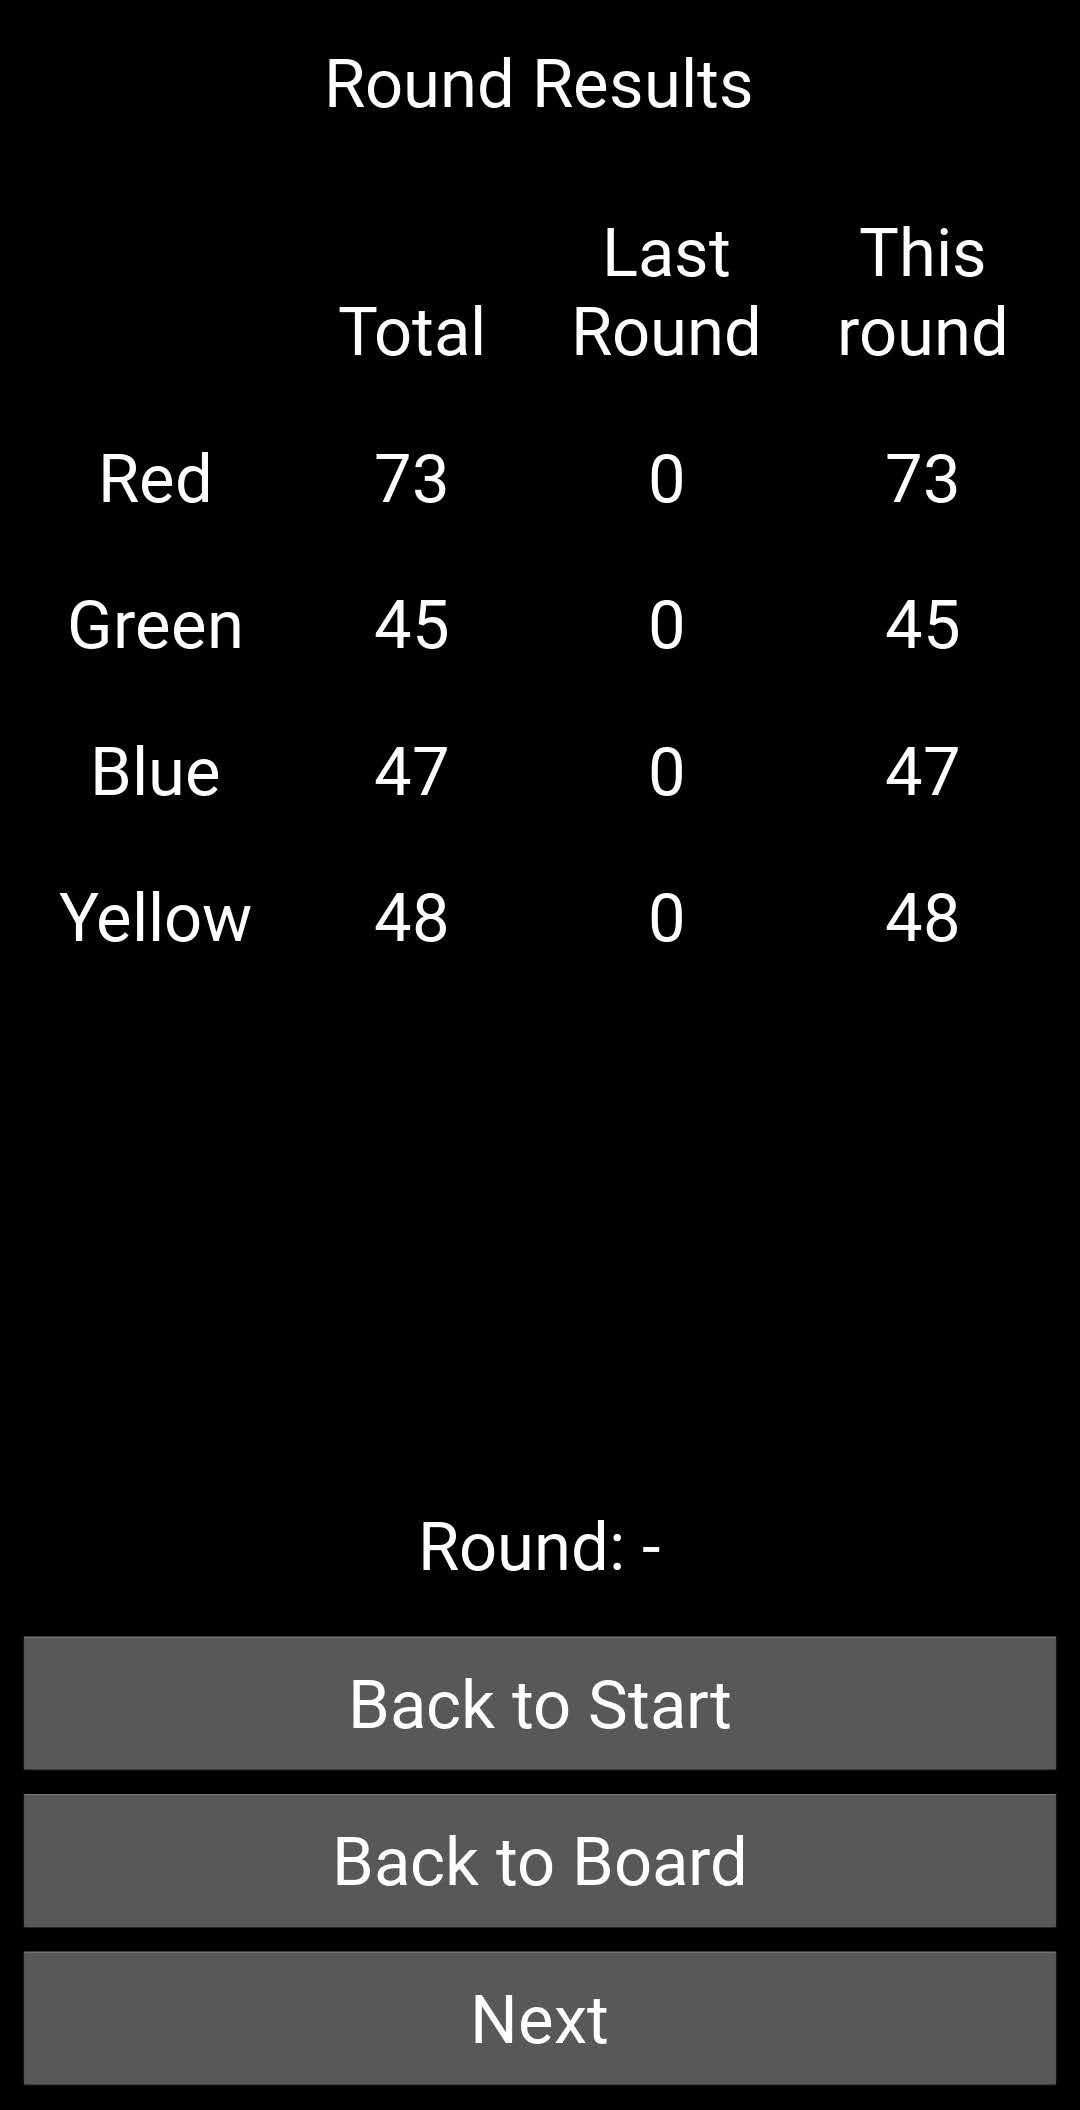
\includegraphics[width=\linewidth]{figures/player_scores.jpg}
				\caption{Zaslon s prikazanim bodovima svakog igrača.}
				\label{podslk:bodovi}
			\end{subfigure}
			
			\caption{Najvažniji zasloni Android aplikacije.}
			\label{slk:zasloni_aplikacije}
		\end{figure}
		
		Drugi način rada funkcionira na isti način kao i prvi, ali ne prati ukupan rezultat igre kroz tri runde. Ovaj režim dakle radi analizu stanja igre u samo jednom trenutku, dakle nad samo jednom fotografijom. Nakon analize jednog stanja igre aplikacija se vraća na početni zaslon sa slike~\ref{slk:zasloni_aplikacije}a.

		\subsection{Programski jezik i radni okvir za razvoj aplikacije}
			Iako je za razvoj Android mobilnih aplikacija danas prema Googleu preferiran programski jezik Kotlin~\cite{IBMChoosingLanguage}, u ovom je projektu korišten programski jezik Python. Glavni razlog za takvu odluku je činjenica da je kod za detekciju ploče korišten za izradu skupa podataka za učenje već bio napisan u Pythonu uz korištenje  biblioteke \textit{OpenCV}. Taj isti kod je također potreban za rad aplikacije prilikom detekcije ploče na fotografiji koju korisnik daje aplikaciji. Sama biblioteka \textit{OpenCV} je dostupna i za programski jezik Java, koji je interoperabilan s Kotlinom~\cite{IBMChoosingLanguage}. No, tada bi za razvoj aplikacije u programskom jeziku Kotlin bilo potrebno dio koda za detekciju ploče prevoditi iz programskog jezika Python u Kotlin, što bi bio nepotreban posao koji ne doprinosi ničemu. Alternativa bi bila pokretanje postojećeg Python koda unutar Kotlin aplikacije s pomoću alata \textit{Chaquopy}~\cite{PowerGatePythonAndroidDiscussion}, ali ta varijanta je djelovala jako nespretno te je s toga odbačena kao mogućnost.
			
			S obzirom na to da Python nema nativnu podršku za Android, za razvoj mobilne aplikacije je korišten radni okvir \textit{Kivy}. \textit{Kivy} je radni okvir otvorenog koda koji omogućuje razvoj aplikacija za razne platforme~\cite{PowerGatePythonAndroidDiscussion}. Dakle s pomoću ovog radnog okvira moguće je razviti aplikaciju za razne operacijske sustave kao što su Windows, iOS, Android, Linux i drugi. No u ovom radu je fokus bio isključivo na razvoju aplikacije za Android. 
			
			Zbog korištenja radnog okvira \textit{Kivy} razvijena aplikacija nema toliko nativan dizajn, ali to za ovaj rad nije bilo pretjerano bitno. Dodatno, mobilne aplikacije razvijane u programskom jeziku Python obično imaju veće memorijsko zauzeće te djeluju nešto sporije od onih razvijenih u programskim jezicima Java i Kotlin. No, rezultantna aplikacija je imala solidne performanse i relativno veliko, ali još uvijek razumno memorijsko zauzeće.
		
		\subsection{Radni okvir za korištenje klasifikacijskih modela}
			Nakon odabira programskog jezika i radnog okvira za razvoj aplikacije slijedi novi problem. Naime, ciljana aplikacija mora koristiti modele iz poglavlja~\ref{pog:klasifikacija} koji su izrađeni pomoću biblioteke \textit{PyTorch}. No, zbog načina na koji se \textit{Kivy} aplikacija priprema za Android biblioteka \textit{PyTorch} se ne može koristiti jer ona nije službeno podržana u Android okruženju~\cite{RedditPyTorchForKivyAndroid}. Konkretno, ne postoji službeni recept za pripremu biblioteke \textit{PyTorch} za Android okruženje~\cite{RedditPyTorchForKivyAndroid}. Iako se potreban recept može samostalno izraditi~\cite{GitHubPyTorchForKivyAndroid}, to bi vjerojatno zahtijevalo više iskustva i vremena, a rezultat bi vjerojatno bio lošiji. Zbog navedenoga nije moguće direktno koristiti \textit{PyTorch} modele u \textit{Kivy} Android aplikaciji.
			
			Dakle, potrebno je pronaći alternativan način za korištenje \textit{PyTorch} modela. Postoje tri rješenja za korištenje dubokih modela u mobilnom okruženju koja su se najčešće pojavljivala prilikom istraživanja ovog problema, a to su \textit{PyTorch Mobile}, \textit{TensorFlow Lite} i \textit{ONNX Runntime}. Iako \textit{PyTorch Mobile} djeluje kao prirodan odabir koji direktno proizlazi iz radnog okvira \textit{PyTorch}, glavna mana ovog radnog okvira su lošije performanse modela u odnosu na druge radne okvire~\cite{DzoneTFLitevsONNXvsPyTochMobile}. Konkretno, modeli koji se koriste s pomoću radnog okvira \textit{PyTorch Mobile} obično budu memorijski veći, sporiji te imaju veću potrošnju energije~\cite{DzoneTFLitevsONNXvsPyTochMobile}. Sljedeća opcija, \textit{TensorFlow Lite}, bi trebala davati najbolje performanse u smislu brzine, veličine modela i potrošnje energije~\cite{DzoneTFLitevsONNXvsPyTochMobile} te je često preporučivana opcija. Međutim, prilikom prilagodbe \textit{PyTorch} modela za \textit{TensorFLow Lite} potrebno je te modele prvo izvesti u format ONNX koji služi kao most između raznih radnih okvira za razvoj modela strojnog učenja~\cite{OnnxExplained}. Model se zatim iz formata ONNX može jednostavno izvesti u format za radni okvir \textit{TensorFlow} te učitati i koristiti pomoću radnog okvira \textit{TensorFlow Lite}. No, s obzirom na to da put prilagodbe modela za \textit{TensorFlow Lite} ide preko formata ONNX, radi pojednostavljenja i skraćivanja ovog procesa odlučeno je koristiti radni okvir \textit{ONNX Runntime} koji omogućuje direktno korištenje modela u formatu ONNX~\cite{OnnxExplained}.
		
		\subsection{Korištenje kamere i pristup galeriji mobitela}
			Tijekom razvoja mobilne aplikacije korištenje kamere te učitavanje fotografija iz galerije mobitela unutar aplikacije pokazalo se vrlo izazovnim. Radni okvir \textit{Kivy} nudi određena rješenja za korištenje kamere i galerije, ali ona su se pokazala vrlo nespretna i nepraktična. Konkretno, nakon detaljnog istraživanja ove teme jedino pronađeno rješenje za fotografiranje s pomoću kamere unutar radnog okvira \textit{Kivy} bilo je tako da se napravi snimka zaslona za vrijeme prijenosa slike s kamere uživo. To rješenje, osim što daje nekvalitetnu sliku, je također staro te je sama implementacija zbog istog komplicirana. S druge strane, pristup fotografijama na mobitelu je nešto jednostavniji, ali je vrlo nepraktičan. Problem je u tome da je pregled fotografija moguć kao pregled datoteka u datotečnom sustavu. To na primjer znači da na mobitelu s velikom količinom slika u istoj mapi pregled istih zahtjeva učitavanje opisa svih slika u toj mapi, što može biti vrlo sporo i nepraktično.
			
			Konačno rješenje koje je na kraju izabrano koristi nativne aplikacije za kameru i pregled galerije mobitela. Kako bi se to ostvarilo, potrebno je koristiti takozvani \textit{Intent}. Ukratko, \textit{Intent} je objekt s pomoću kojeg se može zatražiti određena akcija druge komponente ili aplikacije~\cite{AndroidIntent}. S obzirom na to da se radi o mehanizmu vezanom za Android okruženje, on je dostupan u programskim jezicima Java i Kotlin, ali ne i u programskom jeziku Python. Međutim, pomoću biblioteke \textit{PyJNIus}, ranije zvane \textit{JNIus}, moguće je pristupiti Java klasama s pomoću Javinog nativnog sučelja (\textit{engl. Java Native Interface (JNI)}) unutar Python koda~\cite{GitHubPyJNIus}. Ovo se pokazalo kao vrlo elegantno rješenje za jednokratno fotografiranje unutar aplikacije ili odabir fotografije iz galerije mobitela.
		
		\subsection{Alat \textit{Buildozer}}
			Kako bi se razvijena aplikacija mogla instalirati na mobitel, potrebno je izraditi takozvanu APK-datoteku. APK je standardni datotečni format koji se koristi za instalaciju i pokretanje aplikacija na Android operacijskom sustavu~\cite{KasperskyAPK}. Datoteka tipa APK sadrži sve ključne informacije potrebne da aplikacija radi ispravno, uključujući:
			\begin{itemize}
				\item informacije iz manifesta, poput naziva, verzije i prava pristupa,
				\item sredstva (\textit{engl. assets}) i datoteke resursa,
				\item direktorij za pohranu informacija o resursima,
				\item kompiliran kod i izvorne (nativne) biblioteke~\cite{KasperskyAPK}.
			\end{itemize}
			
			Kao najbolje rješenje za izradu datoteke tipa APK pokazao se alat \textit{Buildozer}. \textit{Buildozer} je razvojni alat za pretvaranje Python aplikacija u binarne pakete koji se mogu instalirati na raznim platformama, uključujući i Android uređaje~\cite{BuildozerDocker}. Za izradu datoteke tipa APK potrebno je napraviti datoteku \textit{buildozer.spec} koja sadrži ime, verziju, ovisnosti i postavke aplikacije~\cite{BuildozerDocker}. Alat \textit{Buildozer} održava tim koji je razvio i radni okvir \textit{Kivy} te je stoga i kompatibilan za rad s istim, iako nije ograničen na rad samo s tim radnim okvirom~\cite{BuildozerDocker}. Za jednostavnije korištenje alata \textit{Buildozer} on je korišten unutar \textit{Docker} kontejnera.
			
		\subsection{Rezultantna aplikacija}
			Konačna mobilna aplikacija dakle omogućuje automatsku analizu stanja igraće ploče društvene igre Kraljevstva na temelju ulazne fotografije. Fotografija može biti snimljena kamerom mobilnog uređaja ili odabrana iz galerije. Za oba načina koriste se nativne aplikacije uređaja. Nakon učitavanja slike aplikacija provodi detekciju i ispravljanje igraće ploče, izrezivanje pojedinih polja, klasifikaciju elemenata korištenjem kaskadno povezanih dubokih modela te izračun bodova u skladu s pravilima igre. Cjelokupna obrada izvodi se lokalno na mobilnom uređaju, bez potrebe za internetskom vezom ili korištenjem vanjskih servisa.
			
			Instalirana aplikacija zauzima približno 150 MB prostora za pohranu. Za aplikaciju ove namjene to nije malo, ali glavni razlozi za to su razvoj u programskom jeziku Python te lokalno korištenje modela zbog kojih je bilo potrebno uvesti dodatne vanjske pakete i ovisnosti u APK-datoteku. Brzina izvođenja aplikacije nije bila direktno mjerena. No, kada je aplikacija testirana na mobitelu Samsung Galaxy A55, performanse su bile zadovoljavajuće te je odgoda prilikom detekcije ploče i klasifikacije objekata bila u razumnim okvirima. No, ovakav pristup omogućio je rad bez mrežne povezanosti, uklonjena je ovisnost o vanjskoj infrastrukturi te doprinosi zaštiti privatnosti korisnika jer se fotografije ne šalju na udaljene poslužitelje.
			
			Dodatno vrijedi napomenuti da je prilikom testiranja same aplikacije uočeno je zanimljivo odstupanje u ponašanju sustava. Naime, u pojedinim slučajevima modeli integrirani u mobilnu aplikaciju daju pogrešne predikcije nad primjerima za koje su tijekom treniranja, validacije i testiranja u razvojnom okruženju ostvarivali točne rezultate. Kako bi se isključila mogućnost utjecaja procesa konverzije modela, provedena je usporedba između izvornih \textit{PyTorch} modela i njihovih inačica izvezenih u format ONNX. No, kod usporedbe nije uočena nikakva razlika u predikcijama modela. Stoga se može zaključiti da uzrok odstupanja u predikciji nije sama konverzija modela u format ONNX, već je riječ o drugom čimbeniku čiji uzrok tijekom izrade ovog rada nije utvrđen. Unatoč ovom neuobičajenom problemu, aplikacija još uvijek daje dovoljno dobre predikcije da njezino korištenje ima smisla. Mogućnost da korisnik može ispraviti predikciju modela unutar aplikacije dodatno umanjuje funkcionalne posljedice ovog problema.
			
%-------------------------------------------------------------------------------


%--- ZAKLJUČAK / CONCLUSION ----------------------------------------------------
\chapter{Zaključak}
\label{pog:zakljucak}

	U ovom je radu razmatran problem razvoja mobilne aplikacije za analizu stanja igraće ploče društvene igre Kraljevstva te praćenje rezultata same igre. Cilj rada je razviti mobilnu aplikaciju koja može ovaj zadatak rješavati potpuno lokalno, bez potrebe za vanjskim servisima i internetskom vezom. U tu je svrhu razvijen cijeli programski sustav koji se sastoji od potpornog koda za razvoj te same mobilne aplikacije. Razvijeni programski sustav sastoji se od:
	\begin{itemize}
		\item sustava za detekciju i ispravljanje ploče te izrezivanje pojedinačnih polja, korištenog u aplikaciji i prilikom izrade skupa podataka za učenje,
		\item jednostavne aplikacije za označavanje podataka za učenje,
		\item skupa podataka za učenje,
		\item potpornog programskog koda za rad sa skupom podataka za učenje,
		\item programskog koda za augmentaciju podataka,
		\item dizajna klasifikacijskih modela i njihovih komponenti,
		\item programskog koda za treniranje, testiranje i izvoz klasifikacijskih modela,
		\item logikom za bodovanje igrača u društvenoj igri,
		\item mobilne aplikacije za Android uređaje koja enkapsulira istrenirane modele, logiku igre i sustav za detekciju ploče.
	\end{itemize}
	
	Razvijeni modeli postižu vrlo visoke performanse - većina modela ima savršenu točnost na cijelom skupu podataka za učenje. Mobilna aplikacija ostvaruje funkcionalnosti koje su bile zamišljene uz razumne memorijske i vremenske resurse. Uspješno je ostvareno lokalno korištenje klasifikacijskih modela na ograničenim resursima mobilnih uređaja.
	
	Valja napomenuti da postoje i slabe točke u razvijenom sustavu. Prije svega, zbog ograničenog skupa podataka za učenje validacijski i testni skupovi su dosta mali, pogotovo za neke od više specijaliziranih klasifikacijskih zadataka. Zbog toga treba biti svjestan da su procijenjene točnosti vjerojatno previše optimistične te ih treba uzeti sa zrnom soli. Dodatno, tijekom razvoja uočena su određena odstupanja između ponašanja klasifikacijskih modela u razvojnom okruženju i u mobilnoj aplikaciji. Sam uzrok tog odstupanja nije u potpunosti razjašnjen u ovom radu.
	
	Za budući rad postoji nekoliko smjerova u kojima bi se ovaj rad mogao unaprijediti. Jedan od mogućih smjerova daljnjeg razvoja je rad na povećanju skupa podataka za učenje te nadogradnja sustava za označavanje podataka za još brže i lakše označavanje podataka. Na primjer, za brže označavanje većeg skupa podataka mogli bi se koristiti postojeći klasifikacijski modeli te se kasnije samo ispravljati pogrešno klasificirani primjeri. Nadalje, vrijedi istražiti dodatne naprednije tehnike računalnog vida kako bi se postigle bolje performanse nekih klasifikacijskih modela koji nisu ostvarili savršenu točnost ili za koje se na većem skupu podataka pokaže da nemaju savršenu točnost. Također, jedan od ključnih smjerova za daljnju rad bilo bi istraživanje uzroka različitog ponašanja klasifikacijskih modela u razvojnom okruženju i unutar mobilne aplikacije. Još jedan smjer koji vrijedi razmotriti jest moguće nadogradnje za samu aplikaciju, kao na primjer korištenje video toka uživo umjesto snimanja pojedinačnih fotografija. Dodatno, valjalo bi razviti i verzije aplikacije prilagođene za druge platforme, kao naprimjer za iOS. S obzirom na to kako je aplikacija razvijena, takav korak bi zahtijevao relativno male izmjene koje se tiču isključivo specifičnosti vezanih za konkretne operacijske sustave.

% Daljnji razvoj aplikacije - više mogućnosti, bolje sučelje

% Pronaći bug

% Razmotriti korištenje jednog modela, dijeljenje značajki, druge arhitekture i dizajne modela...



%--- LITERATURA / REFERENCES ---------------------------------------------------

% Literatura se automatski generira iz zadane .bib datoteke / References are automatically generated from the supplied .bib file
% Upiši ime BibTeX datoteke bez .bib nastavka / Enter the name of the BibTeX file without .bib extension
\bibliography{literatura}


%--- SAŽETAK / ABSTRACT --------------------------------------------------------

% Sažetak na hrvatskom
\begin{sazetak}
	Ovaj rad opisuje razvoj sustava za automatsko bodovanje društvene igre Kraljevstva korištenjem metoda računalnog vida i dubokog učenja. Cilj rada bio je omogućiti jednostavan prijenos stanja igre s fizičke igraće ploče u digitalni oblik te automatizirati proces izračuna bodova kroz Android mobilnu aplikaciju.
	
	Razvijen je algoritam za detekciju uglova igraće ploče na fotografiji, perspektivnu transformaciju slike te izdvajanje pojedinačnih polja ploče. Za prepoznavanje elemenata igre izrađen je skup podataka dobiven fotografiranjem stvarnih konfiguracija ploče te je dodatno pojačan metodama augmentacije podataka radi povećanja robusnosti modela. Implementirano je više konvolucijskih neuronskih mreža koje kaskadnim odlučivanjem klasificiraju različite vrste objekata na ploči, uključujući prazna polja, dvorce, kartice s brojevima i posebne kartice.
	
	Uz sustav računalnog vida razvijen je i programski model pravila igre koji omogućuje automatski izračun bodova na temelju prepoznatog stanja ploče. Cjelokupna funkcionalnost integrirana je u Android mobilnu aplikaciju koja sav izračun obavlja lokalno na uređaju bez potrebe za vanjskim poslužiteljima. Rezultati pokazuju da razvijeni sustav uspješno prepoznaje elemente igre i omogućuje učinkovitu automatizaciju procesa bodovanja.

\end{sazetak}

\begin{kljucnerijeci}
	računalni vid, duboko učenje, konvolucijske neuronske mreže, obrada slike, Android aplikacija, društvene igre, Kraljevstva.
\end{kljucnerijeci}


% Abstract in English
\begin{abstract}
	This thesis presents the development of an automated scoring system for the board game Kingdoms using computer vision and deep learning techniques. The objective was to enable a simple transfer of game state information from a physical game board into a digital representation and to automate the score calculation process through an Android mobile application.
	
	A board detection algorithm was developed to locate the corners of the game board in a photograph, perform perspective transformation, and extract individual board positions. A dataset was created by photographing real game configurations, while various data augmentation techniques were applied to improve model robustness. Several convolutional neural networks were implemented, using a cascading decision-making process to classify different types of objects on the board, including empty cells, castles, numbered cards, and special cards.
	
	In addition to the computer vision subsystem, an implementation of the game rules was developed to calculate scores based on the board state. The complete solution was integrated into an Android application that performs all computations locally without relying on external servers. The results demonstrate that the proposed system successfully recognizes game elements and provides effective automation of the scoring process.

\end{abstract}

\begin{keywords}
	computer vision, deep learning, convolutional neural networks, image processing, Android application, board games, Kingdoms.
\end{keywords}


%--- PRIVITCI / APPENDIX -------------------------------------------------------

% Sva poglavlja koja slijede će biti označena slovom i riječi privitak / All following chapters will be denoted with an appendix and a letter
\backmatter
\chapter{Radni okvir za izradu skupa podataka i klasifikacijskih modela}
\label{appendix:dataset_and_model_framework}

	U ovom privitku je detaljnije objašnjeno kako koristiti kompletan izvorni kod koji je korišten u ovom radu. Sav izvorni kod zajedno sa skupom podataka za učenje je dostupan u GitHub repozitoriju na ovoj \href{https://github.com/PetarBelosevic/KingdomsApp}{poveznici}. Za rad s izvornim kodom potrebno je smjestiti se u direktorij \textit{code} Git repozitorija.
	
	\subsection{Rad sa skupom podataka za učenje}
		U ovom poglavlju je detaljno objašnjeno kako koristiti izvorni kod za rad sa skupom podataka za učenje. To uključuje njegovu izradu, označavanje, podjelu, filtriranje, računanje statistika, pregled karakteristika skupa podataka te korištenje augmentacija.

		\subsection{Generiranje primjera za skup podataka za učenje}
			Za izradu skupa podataka prvo je potrebno imati fotografije igraće ploče iz kojih će se izraditi skup podataka. Njih je potrebno spremiti u direktorij \textit{dataset/board/original\_board\_images}. 
			
			Sljedeće je potrebno pokrenuti skriptu \textit{dataset\_framework/image\_cropper.py}. Skripta koristi kod za detekciju, ispravljanje i izrezivanje ploče koji se nalazi u direktoriju \textit{board}. Prilikom pokretanja skripta obrađuje samo jednu sliku, stoga ju je potrebno pokrenuti više puta kako bi se svaka slika obradila. Dodatno, predefinirano ponašanje skripte je da se rezultat ne sprema. Razlog tome je da se korisniku omogući provjera ispravnosti detekcije ploče prije spremanja. Stoga je uputno za svaku sliku prvo pokrenuti skriptu bez uključene opcije spremanja, a tek nakon što je valjanost detekcije potvrđena ponovno pokrenuti skriptu s uključenom opcijom spremanja. Opcija spremanja se mijenja na kraju skripte kod poziva funkcije \textit{process\_new\_board\_image}. Alternativno se na kraju skripte može pozvati funkcija \textit{iterate\_all\_images} koja će prikazati rezultat svake slike bez spremanja. Nakon toga se skripta može ponovno pokretati uz pozivanje funkcije \textit{process\_new\_board\_image} uz uključenu opciju spremanja. Slika ispravljene ploče bit će spremljena u direktorij \textit{dataset/board/rectified\_boards}, dok će izrezana polja biti spremljena u direktorij\\\textit{dataset/cells/original\_cell\_images}. Ako se želi pregledati međurezultate obrade svake slike potrebno je podesiti argument \textit{show\_intermediate} na vrijednost \textit{True} kod poziva jedne od spomenutih funkcija.
			
		\subsection{Označavanje podataka}
			Za označavanje podataka dovoljno je pokrenuti skriptu\\\textit{dataset\_framework/labeling/labeling\_ui\_shortcuts.py} koja će otvoriti aplikaciju za označavanje. Aplikacije omogućava označavanje neoznačenih podataka te pregledavanje oznaka već označenih podataka. Samo sučelje je vrlo jednostavno te je već ranije prikazano na slici~\ref{slk:oznacavanje}. Oznake se spremaju u datoteku \textit{dataset/cells/original\_cell\_images/labels.json}.
		
		\subsection{Podjela podataka i generiranje pogleda}
			Nakon što su svi podaci označeni, dovoljno je pokrenuti skriptu \textit{dataset\_framework/split\_dataset.py} kako bi se napravila podjela na skup za treniranje, validacijski skup te testni skup. Za eventualno konfiguriranje drugačijeg omjera veličine skupa za treniranje, validacijskog i testnog skupa potrebno je zadati parametar \textit{train\_valid\_test\_ratios} prilikom pozivanja funkcije \textit{split\_dataset\_by\_classes}. Za svaki podskup podataka generira se pripadni direktorij: \textit{dataset/train\_set}, \textit{dataset/validation\_set} i \textit{dataset/test\_set}. U svakom od generiranih direktorija nalazi se datoteka \textit{labels.json} u kojoj su spremljene oznake podataka koji pripadaju tom skupu.
			
			Za generiranje pogleda dovoljno je pokrenuti skriptu \textit{dataset\_framework/generate\_views.py}. Ova skripta će za svaki skup podataka napraviti zasebne poglede kako su opisani u poglavlju~\ref{podpog:podjela_podataka} te za generirane poglede spremiti filtrirane oznake u datoteku\\\textit{views/\{ime\_pogleda\}/labels.json} u pripadnom direktoriju svakog skupa.
			
			U slučaju korištenja normalizacije podataka u modelima moguće je izračunati potrebne srednje vrijednosti i standardne devijacije za svaki pogled u skupu za treniranje. U tu svrhu potrebno je pokrenuti skriptu \textit{dataset\_framework/dataset\_statistics.py}. Skripta će navedene statistike spremiti u datoteku \textit{stats.yaml} u pripadnom direktoriju svakog pogleda u skupu za treniranje. Normalizacija podataka nije bila korištena u radu, ali je ostavljena kao mogućnost radi kompletnosti. 
			
			Konačno se za cijeli skup podataka te svaki podskup može pregledati brojnost primjera svake klase, eventualno nedostajanje primjera iz neke klase te prisutnost nevažećih oznaka. Za to je potrebno pokrenuti skriptu \textit{dataset\_framework/dataset\_validation.py}.
	
		\subsection{Testiranje augmentacija}
			Za pregledavanje i testiranje korištenih augmentacija potrebno je pokrenuti skriptu \textit{dataset\_framework/augmentation/augmentation\_testing.py}. Skripta prvo odabire nasumičnu sliku iz skupa podataka za učenje. Zatim na njoj provodi svaku augmentaciju zasebno, što rezultira prikazom kakav je na slici~\ref{slk:augmentacije_zasebno}. Nakon toga se nad istom slikom generira 36 nasumičnih augmentacija na isti način kako se one primjenjuju prilikom treniranja modela. Rezultat tih 36 augmentacija je vidljiv na slici~\ref{slk:augmentacije_nasumicno}. Konačno se prikazuje augmentacija dodavanja obje vrste sjena. Za svaku vrstu sjena odabire se slučajna slika te se nad njom primjenjuje augmentacija dodavanja te vrste sjene 24 puta.
	
	\section{Rad s klasifikacijskim modelima}
		Implementacije klasifikacijskih modela i njihovih gradivnih blokova, kako su opisani u poglavlju~\ref{podpog:arhitektura_modela}, dostupne su u direktorijima \textit{models} i \textit{models/base}.
		
		Za potrebe treniranja svaki model ima pripadni direktorij nazvan po imenu tog modela smješten u direktoriju \textit{training/experiments}. U direktoriju svakog modela spremljena je konfiguracija treniranja tog modela u datoteci \textit{config.yaml} koja između ostalog sadrži hiperparametre treniranja iz tablice~\ref{tab:cnn_hiperparametri}. Dodatno, direktorij modela služi za spremanje podataka vezanih uz svako pokretanje treniranja modela. To uključuje arhitekturu modela, mjerene gubitke za skupu za treniranje i validacijskom skupu, točnost na validacijskom skupu te parametre modela za svaku epohu treniranja.
		
		Za pokretanje samog treniranja potrebno je pokrenuti skriptu \textit{training/train.py}. Za odabir modela koji će se trenirati potrebno je u skripti podesiti ispravno ime modela kao argument \textit{model\_name} kod pozivanja funkcije \textit{load\_configuration}. Na kraju treniranja skripta otvara prikaz za pregled podataka za odrađena treniranja tog modela u web pregledniku. Time je omogućen jednostavan pregled korištenih arhitektura, točnosti i gubitka na validacijskom skupu te gubitka na skupu za treniranje kroz epohe kako bi se jednostavno odabrali optimalni parametri modela. Kako bi se odabrani model vrednovao potrebno je u skripti \textit{training/test.py} ponovno podesiti ispravno ime modela kao argument \textit{model\_name} kod pozivanja funkcije \textit{load\_configuration} te postaviti varijable \textit{run\_num} na indeks pokretanja treniranja i \textit{epoch} na epohu za odabrane parametre modela. Nakon toga se skripta može pokrenuti. Skripta će ispisati mjere vrednovanja iz poglavlja~\ref{podpog:odabir_i_vrednovanje} te prikazati pogrešno klasificirane primjere na testnom skupu ako takvi postoje.
		
		Kako bi se odabrani modeli izvezli u format ONNX potrebno je u skripti\\\textit{training/model\_exporting.py} zadati ispravne vrijednosti indeksa pokretanja i epohe za odabrane modele u varijabli \textit{BEST\_MODEL\_RUN\_EPOCH}. Nakon toga je dovoljno pokrenuti skriptu. Izvezeni modeli će biti spremljeni u direktorij \textit{mobile\_app/onnx\_models}. Kako bi se provjerila ispravnost izvezenih modela, može se pokrenuti skripta\\\textit{training/validate\_onnx\_export.py}. Skripta za svaki izvezeni model provjerava ako su njegove predikcije jednake predikcijama njegovog originalnog para na cijelom skupu podataka za učenje.
	
	\section{Mobilna aplikacija}
		Sav kod i resursi koje mobilna aplikacija direktno koristi nalaze se u direktoriju \textit{mobile\_app}. To uključuje glavnu logiku aplikacije, njezin dizajn, klasifikacijske modele u formatu ONNX, spremljene podatke o tekućoj igri, kod za procesiranje slike prilikom detekcije ploče, logiku društvene igre, pristup kameri i galeriji Android uređaja te upravljanje klasifikacijskim modelima. Ovdje se također nalazi \textit{buildozer.spec} datoteka koja je ključna za izradu datoteke tipa APK ove aplikacije.
		
		Za izradu nove datoteke tipa APK potrebno je pokrenuti \textit{Docker} kontejner za alat \textit{Buildozer} s kopiranim sadržajem direktorija \textit{mobile\_app} te pričekati da se datoteka izgradi. za detaljnije upute može se pogledati službena \href{https://hub.docker.com/r/kivy/buildozer}{dokumentacija} pripadne \textit{Docker} slike. U slučaju ponovnog pokretanja \textit{Docker} kontejnera radi ispravljanja grešaka u aplikaciji preporučljivo je izbrisati prethodno generirane pomoćne datoteke i direktorije koji su nastali kao nusprodukt izgradnje datoteke tipa APK.
	



% \Blindtext


\end{document}
